\section{\chatextfolModels}\label{cha:folModels}

We now extend the tensor representation to structured representations, whereas the above was on factored representation of systems.
The models/events in this situation are precise relations between objects.





%
\subsection{World Tensors}

\red{We introduce here object enumerating variables $\indvariable$ are valued in $[\inddim]$, with $\cardof{\worlddomain} = \inddim$ and an enumeration of $\worlddomain$ by $\exindividualof{\indindex}$.}

% Formulas in FOL
Formulas in first order logic can contain variables, which are placeholder for specific individuals.
Given a model and an assignment of objects to the arguments of a formula, the truth of the formula can be interpreted.
This truth interpretation defines thus for any model a tensor, which we call the grounding tensor.

% Assumptions
Let us assume, that we have a function-free theory with $\folpredicateorder$ predicates, where are predicates all of the same arity $\variableorder$.
We then formalize a world in the following based on a selection variable $\selvariable$ selecting a specific predicate and term variables $\shortindvariablelist=\indvariablelist$ representing choices of objects from a given set $\worlddomain$.

\begin{definition}[FOL World]
	Given a set of objects $\worlddomain=\{\exindividualof{\indindex} \, : \, \indindexin\}$ enumerated by $[\inddim]$ and a finite set $\{\folpredicates\}$ of $\variableorder$-ary predicates a world is a Boolean tensor
	\begin{align}
		\dataworldat{\selvariable,\indvariableof{[\indorder]}} : [\folpredicateorder] \times \left( \bigtimes_{\indenumeratorin} [\inddim] \right) \rightarrow [2] \, . 
	\end{align}
	
	We interpret the world tensor as encoding in the coordinate $\dataworldat{\selvariable=\folpredicateenumerator,\indexedindvariableof{[\indorder]}}$, whether the substitution of the variables in the $\folpredicateenumerator$th predicate by the individuals $\individuals$ is satisfed on a corresponding world, that is
	\begin{align*}
		\folpredicateof{\folpredicateenumerator}(\individuals) = \dataworldat{\selvariable=\folpredicateenumerator,\indexedindvariableof{[\indorder]}} \, . 
	\end{align*}
\end{definition}


% Inclusion of functions, predicates of differing order
When the assumptions are not met, we can do the following tricks.
Functions are turned to predicates by their relation interpretation.
If there are predicates of different arity in the theory, we can trivially extend them to $\variableorder$ary predicates by tensor products with the trivial tensor $\ones$.
This can be done by a tensor product with $\onehotmapofat{0}{\indvariable}$, where we add an object $\exindividualof{0}$ as a placeholder for predicates with smaller arity.

% Finite worlds -> By database semantics?
While in first order logics, depending on the chosen semantics, worlds can have infinite sets of objects, we here only treat worlds with finite objects.

%\red{Support only Worlds with finite objects!}

\subsubsection{Special Case of Propositional Logics}

% 
Propositional Logics is the case of $\indorder=0$.
In that case, worlds are
	\[ \dataworld: [\folpredicateorder] \rightarrow [2] \]
and represented by the tuples $\atomlegindexof{\atomenumerator} = \dataworld(\atomenumerator)$ as before.

% Comparison with PL
Compared with propositional formulas, the grounding tensor does not take as input a specific world, but is defined on a given world.
We show in this chapter, how both tensor interpretations can be transformed, i.e. by extracting samples from a FOL world $\dataworld$ interpretated as an empirical distribution over PL worlds, and by generating FOL worlds by a set of samples generated from a PL distribution.


\subsubsection{Enumeration of worlds}

%\red{Database semantics here! Enumerate the worlds }

We here enumerate worlds coinciding in their domains. 
This is typical in database semantics, where only those worlds are considered which domains have a one-to-one map to the constant symbols appearing in a knowledge base. % Unique name assumption + Domain closure!
As above we use term variables $\indvariable$ to represent objects in the domain $\worlddomain$ of a world.

% Propositional 
Propositional worlds have been enumerated by indices of $\atomorder$ Booleans, that is for a world $\dataworld: [\folpredicateorder] \rightarrow [2]$ we take the index
	\[ \atomindices \quad \text{where} \quad \atomlegindexof{\atomenumerator} = \dataworld(\atomenumerator) \, .  \]

% FOL
When we want to enumerate the first order logic worlds to a fixed set of objects $\worlddomain$, we flatten the tensor $\dataworld$ and get indices 
	\[ \{\atomlegindexof{\atomenumerator,\indindexlist} \, : \, \atomenumeratorin, \indindexlist \in[\inddim] \} \quad 
	\text{where} \quad \atomlegindexof{\atomenumerator,\indindexlist} = \dataworld(\atomenumerator,\indindexlist) \, .  \]


% Factored systems
When restricting to worlds coinciding in their domain, we still have a factored respresentation of the system, since we can enumerate the possible worlds by a cartesian product.
However, the number of categorical variables representing the world is $\atomorder\cdot \inddim^{\indorder}$ and tensor representations, even in sparse formats, are not feasible due to the large order required.


\subsubsection{Random World Tensors}


\red{Random worlds with fixed domains $\worlddomain$ are probability distributions among possible tensors.}

% Definitions
All possible world tensors given a set of objects $\worlddomain$ are enumerated by a Boolean to each coordinate of the tensor, indicating whether the corresponding assertion holds in the world.
Random worlds are then probability distributions
\begin{align*}
	\probtensor : \bigtimes_{\atomenumeratorin, \, \indindexlist \in[\inddim]} [2] \rightarrow \rr \, . 
\end{align*}

% High-dimensional - watch out for repetitions!
We notice, that by definition these probability distributions are distributions of $\atomorder\cdot\inddim^{\indorder}$ Booleans with $2^{\left(\atomorder\cdot\inddim^{\indorder}\right)}$ many states.
We will later in this chapter investigate methods to handle such high-dimensional distributions in the formalism of exponential families.




\subsection{Formulas in first order logics}

% Arbitrary formulas
Given a FOL World $\dataworld$, arbitrary formulas in first order logics are interpreted in terms of the satisfactions of their groundings.

\begin{definition}[Grounding of FOL Formulas]
	Given a specific world $\dataworld$, with domain $\worlddomain$ enumerated by $[\inddim]$, the grounding of a formula $\folexformula$ with $\individualorder_{\folexformula}$ variables is the tensor
		\[ \groundingofat{\folexformula}{\indvariableof{\folexformula}} :  \bigtimes_{\indenumerator\in[\individualorder_{\folexformula}]} [\inddim] \rightarrow [2] \, . \]
	
	We interpret the coordinates as encoding, whether the substitution of the variables in the formula is satisfied given a world $\dataworld$, that is
	\begin{align*}
		\groundingofat{\folexformula}{\indindexof{0},\ldots,\indindexof{\individualorder_{\folexformula}-1}} = 
			\begin{cases}
				1 \quad \text{if $\folexformula\left(\exindividualof{\indindexof{0}},\ldots,\exindividualof{\indindexof{\individualorder_{\folexformula}-1}}\right)=1$ given the world $\dataworld$}  \\
				0 \quad \text{else}
			\end{cases} \, . 
	\end{align*}
\end{definition}


% Slicing interpretation
Slicing the grounding tensor of a FOL Formula amounts to substitution of the respective variable by the constant at the enumeration index.


% Generic formulas
The above definition of formulas can be interpreted as a map from worlds to grounding tensors
	\[ \folexformula : \dataworld \rightarrow \groundingof{\folexformula} \, . \]
When interpreting this map as a basis encoding, formulas are tensors in the tensor space 
\begin{align*}
 	\left(\bigotimes_{\atomenumeratorin, \indindexlist\in[\inddim]} \rr^{2} \right) \otimes 
	\left(  \bigotimes_{\atomenumeratorin, \indindexof{0},\ldots,\indindexof{\individualorder_{\folexformula}}\in[\inddim]} \rr^{2} \right) \, . 
\end{align*}




% Atomic
Atomic formulas are stored in the slices to the first axis of $\dataworld$ and we have
\begin{align}
	\groundingof{\folpredicateof{\folpredicateenumerator}} = 
	\contractionof{\{\dataworld[\selvariable,\shortindvariablelist], \onehotmapofat{\folpredicateenumerator}{\selvariable}\}}{\shortindvariablelist} \, . 
\end{align}



%\begin{figure}[h]
%	\begin{center}
%		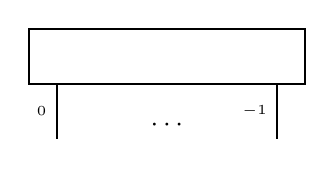
\begin{tikzpicture}[scale=0.35, thick] % , baseline = -3.5pt

    %	\draw[->] (0,1)--(0,3) node[midway,left] {$\atomlegindexof{\exformula}$};
	
    	\draw (-5,1) rectangle (5,-1);
    	\node[anchor=center] at (0,0) {\small ${\groundingof{\exformula}}$} ;
    	\draw[] (-4,-1)--(-4,-3) node[midway,left] {\tiny $\exindividualof{0}$};
    	\draw[] (4,-1)--(4,-3) node[midway,left] {\tiny $\exindividualof{\variableorder-1}$};
    	\node at (0,-3.1) [above] {$\cdots$};
    
\end{tikzpicture}
%	\end{center}
%	\caption{Grounding tensor to a formula $\folexformula$ with $\variableorder$ arguments on world $\dataworld$. }
%	\label{fig:groundingTensor}
%\end{figure}



\subsubsection{Syntactical Decomposition of quantifier-free formulas}

In order to have a sound semantic, the grounding of FOL formulas is determined by the syntax of the formula, i.e. a decomposition of the formula into connectives and quantifiers acting on atomic formulas.

% Formulas as maps from worlds to groundings
Quantifier-free formulas are connectives acting on atomic formulas.
We can describe them as in the case of propositional logics in the $\rencodingof{}$-formalism.
While the atomic formulas where delta tensors copying states, they are more involved here.



\begin{theorem}
	For any connective $\exconnective$ and formulas $\folexformula_1$ and $\folexformula_2$ we have
	\begin{align}
		\groundingof{(\folexformula_1\exconnective\folexformula_2)}[\shortindvariablelist] = 
			\contractionof{\{
			\rencodingofat{\groundingof{\folexformula_1}}{\shortindvariablelist,\catvariableof{\folexformula_1}},
			\rencodingofat{\groundingof{\folexformula_2}}{\shortindvariablelist,\catvariableof{\folexformula_2}},
			\rencodingofat{\exconnective}{\catvariableof{\folexformula_1\exconnective\folexformula_2}, \catvariableof{\folexformula_1}, \catvariableof{\folexformula_2}}, 
			\onehotmapofat{1}{\catvariableof{\folexformula_1\exconnective\folexformula_2}}			
			\}}
			{\shortindvariablelist} \, . 
	\end{align}
\end{theorem}
\begin{proof}
	By the semantic interpretation of the groundings, which has to be sound.
\end{proof}

% Shared variables
Here, variables can be shared by the connected formulas, therefore the variables in the combined formula are unions of the possible not disjoint variables of the connected formulas.

%% Propositional interpretation
%When we understand the head variables in the relational encoding of atoms as the categorical variables, and get a similar interpretation of the tensor network decomposition as in the propositional case.
%\subsubsection{Propositionalization}

When interpreting the head variables of relational encoded atomic formulas as the atoms of a propositional theory, we find a propositional formula $\exformula$ associated with any decomposable first order logic formula.

\begin{definition}\label{def:propositionalEquivalent}
	Given a formula $\folexformula$ in first order logic, we say that a propositional formula $\formulaat{\shortcatvariables}$ is the propositional equivalent to $\folexformula$ given atomic formulas $\extformulaof{\atomenumerator}$ in first order logic, when for any world $\dataworld$ we have
	\begin{align}
		\groundingofat{\folexformula}{\indvariableof{\folexformula}}
		= \contractionof{ 
		\{\rencodingofat{\groundingof{\extformulaof{\atomenumerator}}}{\indvariableof{\extformulaof{\atomenumerator}}, \catvariableof{\atomenumerator}} : \atomenumeratorin\} 
		\cup \{\formulaat{\shortcatvariables} \}
		}{\indvariableof{\folexformula}}
	\end{align}
\end{definition}



We depict the relation of a grounding tensor to a propositional formula 
\begin{center}
	\begin{tikzpicture}[scale=0.35, yscale=1, thick] % , baseline = -3.5pt



%\draw[] (2,-1) -- (2,1) node[midway,left] {\tiny $\atomicformulaof{0}$};
%\node[anchor=center] (text) at (4,0) {$\cdots$};
%\draw[] (6,-1) -- (6,1) node[midway,right] {\tiny $\atomicformulaof{\atomorder-1}$};

\draw (1,-1) rectangle (7,-3);
\node[anchor=center] (text) at (4,-2) {$\groundingof{\folexformula}$};

\draw[] (2,-3) -- (2,-5) node[midway,left] {\tiny $\individualvariableof{0}$};
\node[anchor=center] (text) at (4,-4) {$\cdots$};
\draw[] (6,-3) -- (6,-5) node[midway,right] {\tiny $\individualvariableof{\individualorder-1}$};


\node[anchor=center] (text) at (10,-2) {${=}$};



%\draw (1,-1) rectangle (7,-3);
%\node[anchor=center] (text) at (4,-2) {$\rencodingof{\impformula}$};

\begin{scope}[shift={(12,-2)}]

\draw (1,3) rectangle (12,5);
\node[anchor=center] (text) at (6.5,4) {$\exformula$};

\draw[->] (2.5,1) -- (2.5,3) node[midway,right] {\tiny $\atomicformulaof{0}$};
\draw (1,-1) rectangle (4,1);
\node[anchor=center] (text) at (2.5,0) {$\rencodingof{\groundingof{\extformulaof{0}}}$};
\node[anchor=center] (text) at (2.5,-2) {$\cdots$};

\node[anchor=center] (text) at (6.5,0) {$\cdots$};

\draw[->] (10.5,1) -- (10.5,3) node[midway,right] {\tiny $\atomicformulaof{\atomorder-1}$};
\draw (8.75,-1) rectangle (12.25,1);
\node[anchor=center] (text) at (10.5,0) {$\rencodingof{\groundingof{\extformulaof{\atomorder\shortminus1}}}$};
\node[anchor=center] (text) at (10.5,-2) {$\cdots$};

\draw[-] (11.5,-3) -- (3.5,-3) ;
\draw[-] (9.5,-5) -- (1.5,-5) ;

\draw[fill] (11.5,-3) circle (0.25cm);
\draw[->] (11.5,-3) -- (11.5,-1);

\draw[fill] (9.5,-5) circle (0.25cm);
\draw[->] (9.5,-5) -- (9.5,-1);

\draw[fill] (3.5,-3) circle (0.25cm);
\draw[->] (3.5,-3) -- (3.5,-1);

\draw[fill] (1.5,-5) circle (0.25cm);
\draw[->] (1.5,-5) -- (1.5,-1);


\draw[fill] (7.5,-3) circle (0.25cm);
\draw[<-] (7.5,-3) -- (7.5,-7) node[right] {\tiny $\individualvariableof{\individualorder-1}$} ;

\node[anchor=center] (text) at (6.5,-6) {$\cdots$};

\draw[fill] (5.5,-5) circle (0.25cm);
\draw[<-] (5.5,-5) -- (5.5,-7) node[left] {\tiny $\individualvariableof{0}$} ;


%\draw (13,-2) rectangle (15,-6);
%\node[anchor=center] (text) at (14,-4) {$\rencodingof{\impformula}$};
%\node[anchor=center] (text) at (12,-3.75) {$\vdots$};
%\draw[->] (15,-4) -- (16,-4);
%\draw[] (17,-4) -- (16,-4);
%\draw (17,-3) rectangle (19,-5);
%\node[anchor=center] (text) at (18,-4) {$\tbasis$};

\end{scope}




		


\end{tikzpicture}
\end{center}




\subsubsection{Quantifiers}

%\red{The variables quantified over are dropped i.e. $\indvariableof{\exists_{\indvariableof{\exists}} \folexformula} =\indvariableof{\folexformula}/\indvariableof{\exists}$.}

Existential and universal quantifiers appear in generic first order logic.
They are not representable as linear transform of the respective quantifier-free formula.
Here we represent them as a compositions of contractions with the greater zero function $\greaterzerofunction$ defined as
\begin{align*}
	\greaterzerofunction : \rr \rightarrow [2] \quad, \quad \greaterzeroof{x} = 
	\begin{cases}
		1 &  \text{if  } x > 0\\
		0 & else
	\end{cases} \, .
\end{align*}


\begin{theorem}
	For any formula $\folexformula$ with variables $\shortindvariablelist$ we have
%	\begin{itemize}
%		\item existential quantification 
		\begin{align}
			\groundingofat{\left(\exists_{\exindividualof{\indindexof{0}}}  \folexformula\right)}{\indvariableof{1},\ldots,\indvariableof{\indorder-1}} = 
			\greaterzeroof{
			\sbcontractionof{\groundingof{\folexformula}}{\indvariableof{1},\ldots,\indvariableof{\indorder-1}}
			}
		\end{align}
	and
%	\item universal quantification 
		\begin{align}
			\groundingofat{\left(\forall_{\exindividualof{\indindexof{0}}} \folexformula\right)}{\indvariableof{1},\ldots,\indvariableof{\indorder-1}}= 
			\greaterzeroof{
			\sbcontractionof{\groundingof{\folexformula}}{\indvariableof{1},\ldots,\indvariableof{\indorder-1}}
			- \inddim \cdot \onesat{\indvariableof{1},\ldots,\indvariableof{\indorder-1}}
			} \, . 
		\end{align}
%\end{itemize}
\end{theorem}
\begin{proof}

%	Coordinatewise: Exists is true, when the slice leaving only the zeroth axis has at least one entry, i.e. its sum is greater than equal.
%	Universal is true, when all are one, i.e. the sum is maximal $\inddim$.
	
	We proof the claimed equalities to arbitrary slices of the remaining variables, which amount to arbitrary substitutions of the formulas.
	For any indices $\indindexof{1},\ldots,\indindexof{\indorder-1}$ we have
	\begin{align*}
		\sbcontractionof{\groundingof{\folexformula}}{\indexedindvariableof{1},\ldots,\indexedindvariableof{\indorder-1}}
		= \sum_{\indindexofin{0}} \groundingof{\folexformula}[\indexedindvariableof{0},\ldots,\indexedindvariableof{\indorder-1}] \, . 
	\end{align*}
	The existential quantification with respect to the zeroth variable is satified, when for at least one $\indindexofin{0}$ we have $\groundingof{\folexformula}[\indexedindvariableof{0},\ldots,\indexedindvariableof{\indorder-1}]=1$, which is equal to 
	\begin{align*}
		 \sum_{\indindexofin{0}} \groundingof{\folexformula}[\indexedindvariableof{0},\ldots,\indexedindvariableof{\indorder-1}]  \geq 1
	\end{align*}
	and
	\begin{align*}
		\greaterzeroof{\sum_{\indindexofin{0}} \groundingof{\folexformula}[\indexedindvariableof{0},\ldots,\indexedindvariableof{\indorder-1}] } = 1 \, . 
	\end{align*}
	Combining both equations we get
	\begin{align*}
		\left(\groundingof{\exists_{\exindividualof{\indindexof{0}}}  \folexformula}\right)[\indexedindvariableof{1},\ldots,\indexedindvariableof{\indorder-1}] 
		= \greaterzeroof{
			\sbcontractionof{\groundingof{\folexformula}}{\indexedindvariableof{1},\ldots,\indexedindvariableof{\indorder-1}}
			}
	\end{align*}
	and arrive at the first claim.
	
	To show the second claim, we notice that the universal quantification with respect to the zeroth variable is satisfied, when for all $\indindexofin{0}$ we have $\groundingof{\folexformula}[\indexedindvariableof{0},\ldots,\indexedindvariableof{\indorder-1}]=1$.
	This is equal to 
	\begin{align*}
		 \sum_{\indindexofin{0}} \groundingof{\folexformula}[\indexedindvariableof{0},\ldots,\indexedindvariableof{\indorder-1}]  = \inddim
	\end{align*}
	and 
	\begin{align*}
		\greaterzeroof{\sum_{\indindexofin{0}} \groundingof{\folexformula}[\indexedindvariableof{0},\ldots,\indexedindvariableof{\indorder-1}] - \inddim} = 1 \, . 
	\end{align*} 
	It follows that
	\begin{align*}
		& \left(\groundingof{\forall_{\exindividualof{\indindexof{0}}} \folexformula}\right)[\indexedindvariableof{1},\ldots,\indexedindvariableof{\indorder-1}] \\
			& \quad \quad =  \greaterzeroof{
			\sbcontractionof{\groundingof{\folexformula}}{\indexedindvariableof{1},\ldots,\indexedindvariableof{\indorder-1}}
			- \inddim \cdot \onesat{\indexedindvariableof{1},\ldots,\indexedindvariableof{\indorder-1}}
			}
	\end{align*}
	which establishes the second claim.
\end{proof}




\subsubsection{Basis CP Decomposition}\label{sec:basisCPgrounding}

In many situations grounding cores are sparse and representations as single tensor cores comes with a drastic overhead.
We often encounter sparse grounding, that is
	\[ \sparsityof{\groundingof{\folexformula}} \leq \inddim^{\variableorder_\folexformula} \, . \]
%We notice, that the number of nonzero coordinates in a datacore constructed from a set of $\datanum$ samples (assuming complete observations) satsifies
%	\[ \sparsityof{\datacore} \leq \datanum \, . \]
%Typically we have
%	\[ \datanum <  2^{\atomorder} \]
In this case the basis CP decomposition (see \secref{sec:basisCP}) enables a representation of the grounding with significantly smaller storage demand, see \theref{the:sparseBasisCP}.
We depict the CP decomposition of a formula grounding in Figure~\ref{fig:groundingCP}.


% Standard KB Encoding and Assumptions
Most logical syntaxes make use of the $\ell_0$-sparsity and explicitly store only the known assertions.
The not specified assertions have different interpretation based on the assumptions made.
Under the Closed World Assumption all unspecified assertions are assumed to be false.

\begin{figure}[h]
\begin{center}
	\begin{tikzpicture}[scale=0.35, yscale=-1, thick] % , baseline = -3.5pt





%\drawatomindices{0}{2}


\draw (-1,1) rectangle (5,-1);
\node[anchor=center] (text) at (2,0) {$\groundingof{\exformula}$};

%\draw[->] (2,-1) -- (2,-3) node[midway, right] {\tiny $\atomlegindexof{\exformula}$};
%\draw[] (3,-3) rectangle (1, -5);
%\node[anchor=center] (text) at (2,-4) {\small $\tbasis$};
%\draw[->] (4,-1) -- (4,-3) node[midway, right] {\tiny $\datindex$};
%\draw[dashed] (3,-3) rectangle (5, -5);
%\node[anchor=center] (text) at (4,-4) {\small $\ones$};

\draw[] (0,1) -- (0,3) node[midway,left] {\tiny $\exindividualof{0}$};
\draw[] (1.5,1) -- (1.5,3) node[midway,left] {\tiny $\exindividualof{1}$};
\node[anchor=center] (text) at (2.75,2) {$\cdots$};
\draw[] (4,1) -- (4,3) node[midway,right] {\tiny $\exindividualof{\variableorder\shortminus1}$};

\node[anchor=center] (text) at (7,0) {${=}$};


\begin{scope}[shift={(10,2)}]

\newcommand{\conposseldec}{4.5,-5.5}

\draw[fill] (\conposseldec) circle (0.25cm);
\draw (\conposseldec) -- (4.5,-7.5) node[midway, right] {\tiny $\datindex$};
\draw[] (3.5,-7.5) rectangle (5.5, -9.5);
\node[anchor=center] (text) at (4.5,-8.5) {\small $\ones$};

\draw[<-] (0,1) -- (0,-1) node[midway,left] {\tiny $\exindividualof{0}$};
\draw (-1,-1) rectangle (1, -3);
\node[anchor=center] (text) at (0,-2) {\small $\legcoreof{\exformula,0}$};
\draw[<-] (0,-3) to[bend right=20] (\conposseldec);


\draw[<-] (3,1) -- (3,-1) node[midway,left] {\tiny $\exindividualof{1}$};
\draw (2,-1) rectangle (4, -3);
\node[anchor=center] (text) at (3,-2) {\small $\legcoreof{\exformula,1}$};
\draw[<-] (3,-3) to[bend right=20]  (\conposseldec);

\node[anchor=center] (text) at (6,-2) {$\cdots$};

\draw[<-] (9,1) -- (9,-1) node[midway,left] {\tiny $\exindividualof{\variableorder\shortminus1}$};
\draw (8,-1) rectangle (10, -3);
\node[anchor=center] (text) at (9,-2) {\small $\legcoreof{\exformula,\variableorder\shortminus1}$};
\draw[<-] (9,-3) to[bend left=20]  (\conposseldec);




\end{scope}

		


\end{tikzpicture}
\end{center}
\caption{Basis CP Decomposition of the grounding of $\folexformula$.}
	\label{fig:groundingCP}
\end{figure}





%% MISLEADING? Groundings assume single worlds, whereas Database Semantics a distribution over worlds with fixed set of objects.
%\subsubsection{Database Semantics}
%
%We here employ the DataBase Semantics and assume a finite list of individuals (constants).
%Then the probability distribution is still over all possible worlds (which are in database semantics those with bijections between the constants of the Knowledge Base and objects in the world).
%
%For each model of a FOL we have the following assumptions of Database Semantics:
%\begin{itemize}
%	\item Unique Name Assumption: Injectivity of the interpretation map of constants.
%	\item Domain Closure: Surjectivity of the interpretation map of constants.
%\end{itemize}
%Thus we assume that the interpretation map of each model is a bijection between constants and objects.
%
%
%Given Database Semantics it is thus ensured, that grounding tensors represent all of the semantics of universally quantified formulas.
%
%\begin{remark}[Closed World Assumption]
%	In this approach we typically further assume that the groundings of the formulas are known.
%	This corresponds with the closed world assumption, where any zero entry in the formula tensor is interpreted as a false corresponding substitution.
%\end{remark}



\subsubsection{Example: Queries}

Queries are formulas $\impformula$, which are asked against a specific world $\dataworld$.
Each argument is of such formulas are called projection variables.
The answer of a query is a list of solution mappings from the projection variables to objects in the world, such that the query formula is true.

% CP Decomposition
Answering a query thus corresponds with finding the basis CP Decomposition (see \secref{sec:basisCP}).

% Inefficiency
There are situations, in which the CP Decomposition comes with unnecessary storage overhead compared with other formats.
To be more precise, let us show how Join operations on groundings are represented by contractions.

\begin{definition}
	Let there be a world with individual sets $\indexset_\node$ for $\node\in\nodes$ and groundings $\groundingof{\extformulaof{l}}$ 
		\[ \groundingof{\extformulaof{l}}: \bigtimes_{\node\in\nodes_l} [\inddimof{\node}] \rightarrow [2] \]
	defined on subsets of the individuals sets $\bigtimes_{\node\in\nodes}\indexset_\node$.
	Then their $\mathrm{Join}$ is defined as
		\[ \groundingof{\mathrm{Join}\left(\extformulaof{0},\ldots,\extformulaof{p-1} \right)} = \prod_{l\in[p]} \groundingof{\extformulaof{l}} \, .\]
\end{definition}

%Visualization
We can understand the $\mathrm{Join}$ of groundings by a factor graph, where each grounding is a factor connecting the variables decorating node sets $\nodes_l$.


\begin{theorem}[Joins by Hadamard products]
	For any $\mathrm{Join}$ of grounded formulas we have
		\[ \groundingofat{\mathrm{Join}\left(\extformulaof{0},\ldots,\extformulaof{p-1} \right)}{\indvariableof{\nodes}} = 
		\sbcontractionof{\groundingof{\extformulaof{0}},\ldots,\groundingof{\extformulaof{p-1}}}{\indvariableof{\nodes}} \, . \]
\end{theorem}
\begin{proof}
	Direct
\end{proof}

Thus, we can store the $\mathrm{Join}$ by at most linear in the number of joined formulas demand.
Storing the result by solution maps on the other side can create storage overheads as we show next.

%\begin{theorem}
%	Given a grounding $\groundingof{\folexformula}$ on a world then the minimal rank of a basis CP Decomposition storing $\groundingof{\folexformula}$  is the number of tuples $\{\exindividualof{\node} \, : \, \node\in\nodes \}$ such that
%		\[ \groundingof{\folexformula}(\{\exindividualof{\node} \, : \, \node\in\nodes \}) = 1\, . \]
%\end{theorem}
%\begin{proof}
%	Later in binary+directed Contraction Calculus, where we also define $\ell_0$-norm
%\end{proof}

\begin{example}
	For example take a query with many basic graph patterns with pairwise different projection variables. 
	The global CP Decomposition would come here with an exponential storage overhead compared with storage as a tensor product of CP Decompositions to each Basic graph pattern.
\end{example}


\begin{remark}[Distinguishing from probabilistic queries]
	Let us distinguish the discussion here from those of queries in probabilistic reasoning, which have two main differences.
	First, we ask queries against all possible pairs of variables, instead of asking the probability of satisfaction of a specific formula. 
	Second, since we made the epistemologic assumption of knowing possibilities and not probabilities in logics, a query is answered by a truth value.
	We then only output in the shape of solution mappings the variable assignments where the query formula is true.
 	Thus, the queries here can be thought of as a batch of probabilistic queries with Boolean answers.
	% Alternative -> Later?
	Probabilistic queries can furthermore be understood in terms of the data extraction process described in this section.
	We can ask the query in probabilistic form (decomposed into atomic formulas) on the resulting empirical distribution.
	This results in the ratio of the worlds satisfying the query among those worlds satisfying the extraction query $\impformula$.
\end{remark}


\subsection{Representation of Knowledge Graphs}

Let us now represent a specific fragment of FOL, namely Description Logics which Knowledge Bases are often refered to as Knowledge Graphs.

\subsubsection{Representation as unary and binary predicates}

% Reduction to binary
Atomic formulas in knowledge bases following the OWL standard (thus, especially knowledge graphs) are binary (owl:ObjectProperties) and unary (owl:Class).
%Larger formulas are created by logical connections of these atomic formulas using disjunctions, conjunctions etc.
We enumerate the predicates by $[\folpredicateorder]$, the objects in the domain $\worlddomain$ by $[\inddim]$, and extend the unary predicates to binaries by tensor product with $\onehotmapofat{0}{\indvariable}$ (see discussion above)
A Knowledge Graph on the set $\worlddomain$ of constants (owl:NamedIndividuals) is the tensor
\begin{align*}
	\kg :  [\folpredicateorder] \times [\inddim] \times [\inddim] \rightarrow [2] \, . 
\end{align*}


\subsubsection{Representation as ternary predicate}

% RDF triple: Alternative viewpoint to collection of unary and binary predicates!
Following our notation we understand a Knowledge Graph as a grounding of the rdf triple relation $\rdf$ (being a formula of order 3) on a specific world $\kg$ with individuals $\worlddomain$
\begin{align*}
	\kggroundingof{\rdf} : [\inddim] \times [\inddim] \times [\inddim] \rightarrow [2]
\end{align*}
where
\begin{align*}
	\kggroundingof{\rdf}(\indindexof{s}, \indindexof{p}, \indindexof{o}) =
	\begin{cases}
	1 \quad & \text{if triple $\braket{\indindexof{s}, \indindexof{p}, \indindexof{o}}$ is in Knowledge Graph $\kg$} \\
	0  \quad & \text{else}
	\end{cases} \, .
\end{align*} 


% Sparse representation
Sparse representation of the grounding tensor to a knowledge graph is of central importance, as investigated in \cite{bigerl_tentris_2020}.
We here do basis CP for sparse representation.
Slicing the tensor $\gtensorof{\kg}$ along the predicate axis retrieves specific information about roles and can be efficiently be performed on these formats.
 
The role \rdftype has a specific meaning, since it contains from a DL perspective classifications (memberships of named concepts).
Further slicing the tensor along object axis therefore results in membership lists for specific classes (concepts).
One can thus regard \rdftype as a placeholder for unitary formulas in a space of binary formulas. 

% Approximation of KG Groundings
Approximations of grounding tensors by decompositions leads to embeddings of the individuals such as Tucker, Complex, RESCAL (see \cite{nickel_review_2016}).

% Relational Encoding
For  our purposes of evaluating logical formulas such as $\sparql$ queries we use the relational encoding of the groundings, which are depicted by
 \begin{center}
	\begin{tikzpicture}[scale=0.3, thick] % , baseline = -3.5pt

    \draw[->-] (0,1)--(0,3) node[midway,left] {\tiny $\headvariable$};
    \draw (-3,1) rectangle (3,-1);
    \node[anchor=center] (text) at (0,0) {\small $\rencodingof{\kggroundingof{\rdf}}$};
    \draw[-<-] (-2,-1)--(-2,-3) node[midway,left] {\tiny $\sindvariable$};
    \draw[-<-] (0,-1)--(0,-3) node[midway,left] {\tiny $\pindvariable$};
    \draw[-<-] (2,-1)--(2,-3) node[midway,left] {\tiny $\oindvariable$};

\end{tikzpicture}
\end{center}
 
 
 
 
%\subsubsection{Graph Patterns}
\subsubsection{$\sparql$ Queries}

The $\sparql$ query language is a syntax to express first order logic formulas $\folexformula$.
Given a specific world $\dataworld$, the execution of query is the interpretation $\groundingof{\folexformula}$, typical represented in a sparse basis CP format where each slice represents a solution mapping.

\paragraph{Triple Patterns}

Formulas which are of specific importance are triple patterns:
\begin{itemize}
	\item Unary triple pattern with one variable, representing a formula with a single projection variable.
	 	For the example $\exunarytriple$ see Figure~\ref{fig:triplePatterns}a.
	\item Binary triple pattern with two variables, representing a formula with two projection variables.
		For the example  $\exbinarytriple$ see Figure~\ref{fig:triplePatterns}b.
\end{itemize}

These triples are compositions of slicing operation, here seen as a map from single or two projection variables to the triples $(\exindividualof{\indindexof{s}}, \exindividualof{\indindexof{p}}, \exindividualof{\indindexof{o}})$, with the $\rdf$ formula.


% By 
These slicing operations are performed by contractions with tensors $\psi^{\braket{...}}$, for unary triple patterns of the shape
	\[ \psi : \left( [\folpredicateorder] \times [\inddim] \times [\inddim] \right) \times [\inddim] \rightarrow [2] \]
and for binary
	\[ \psi : \left( [\folpredicateorder] \times [\inddim] \times [\inddim] \right) \times [\inddim] \times [\inddim] \rightarrow [2] \]
defined by identity and basis vectors depending on the type of triple.

In the example $\exunarytriple$ we have
	\[ \psi^{\exunarytriple} = \identity^{\exindividualof{\sindex},?\exindividualof{0}} \otimes \onehotmapof{0} \otimes \identity^{\exindividualof{\oindex},?\exindividualof{1}}   \]


%
The composition $\psi (\psi^T)$ of the matrification of the tensor $\psi$ is a projection.
That means that applying $\psi (\psi^T)$ is the same map as applying once.


\begin{figure}[h]
\begin{center}
		\begin{tikzpicture}[scale=0.3,thick] % , baseline = -3.5pt

    \begin{scope}
        [shift={(0,0)}]

        \node[anchor=center] (text) at (-12,2) {$a)$};

        \begin{scope}
            [shift={(-7,2)}]

            \draw (0,-3) rectangle (-6,-5);
            \draw[<-] (-3,-1)--(-3,-3) node[midway,right] {\tiny $\headvariable$};
            \node[anchor=center] (text) at (-3,-4) {$\rencodingof{\kggroundingof{\exunarytriple}}$};
            \draw[<-] (-3,-5)--(-3,-7) node[midway,left] {\tiny $\provariableof{0}$};

        \end{scope}

        \node[anchor=center] (text) at (-5.5,-2) {${=}$};

        \draw[->] (0,1)--(0,3) node[midway,left] {\tiny $\headvariable$};
        \draw (-4,1) rectangle (4,-1);
        \node[anchor=center] (text) at (0,0) {\small $\rencodingof{\kggroundingof{\rdf}}$};

        \draw (-2,-3) rectangle (-4,-5);
        \draw[<-] (-3,-1)--(-3,-3) node[midway,left] {\tiny $\sindvariable$};
        \node[anchor=center] (text) at (-3,-4) {$\delta$};
        \draw[<-] (-3,-5)--(-3,-7) node[midway,left] {\tiny $\provariableof{0}$};

        \draw (-1,-3) rectangle (1,-5);
        \draw[<-] (0,-1)--(0,-3) node[midway,left] {\tiny $\pindvariable$};
        \node[anchor=center] (text) at (0,-4) {$\onehotmapof{\invrdftypesymbol}$};

        \draw (2,-3) rectangle (4,-5);
        \draw[<-] (3,-1)--(3,-3) node[midway,left] {\tiny $\oindvariable$};
        \node[anchor=center] (text) at (3,-4) {$\onehotmapof{\exaunaryrelation}$};

    \end{scope}


    \begin{scope}
        [shift={(24,0)}]

        \node[anchor=center] (text) at (-13,2) {$b)$};

        \begin{scope}
            [shift={(-8,2)}]

            \draw (0.5,-3) rectangle (-6.5,-5);
            \draw[<-] (-3,-1)--(-3,-3) node[midway,right] {\tiny $\headvariable$};
            \node[anchor=center] (text) at (-3,-4) {$\rencodingof{\kggroundingof{\exbinarytriple}}$};

            \draw[<-] (-2,-5)--(-2,-7) node[midway,right] {\tiny $\provariableof{0}$};
            \draw[<-] (-4,-5)--(-4,-7) node[midway,left] {\tiny $\provariableof{1}$};

        \end{scope}

        \node[anchor=center] (text) at (-5.5,-2) {${=}$};

        \draw[->] (0,1)--(0,3) node[midway,left] {\tiny $\headvariable$};
        \draw (-4,1) rectangle (4,-1);
        \node[anchor=center] (text) at (0,0) {\small $\rencodingof{\kggroundingof{\rdf}}$};

        \draw (-2,-3) rectangle (-4,-5);
        \draw[<-] (-3,-1)--(-3,-3) node[midway,left] {\tiny $\sindvariable$};
        \node[anchor=center] (text) at (-3,-4) {$\delta$};
        \draw[<-] (-3,-5)--(-3,-7) node[midway,left] {\tiny $\provariableof{1}$};

        \draw (-1,-3) rectangle (1,-5);
        \draw[<-] (0,-1)--(0,-3) node[midway,left] {\tiny $\pindvariable$};
        \node[anchor=center] (text) at (0,-4) {$\onehotmapof{\exabinaryrelation}$};

        \draw (2,-3) rectangle (4,-5);
        \draw[<-] (3,-1)--(3,-3) node[midway,left] {\tiny $\oindvariable$};
        \node[anchor=center] (text) at (3,-4) {$\delta$};
        \draw[<-] (3,-5)--(3,-7) node[midway,right] {\tiny $\provariableof{0}$};

    \end{scope}

\end{tikzpicture}
\end{center}
\caption{Triple patterns of $\sparql$ as tensor networks.
	a) Example of unary triple pattern $\exunarytriple$ specifying whether an individual $\exindividualof{1}$ is a member of class $C$.
	b) Example of a binary triple pattern $\exbinarytriple$ specifying whether individuals $\exindividualof{1}$ and $\exindividualof{2}$ have a relation $R$.
		By $\onehotmapof{0},\onehotmapof{C},\onehotmapof{R}$ we denote the one-hot encodings of the enumeration of the resources $rdf:type, C$ and $R$.}
\label{fig:triplePatterns}
\end{figure}




\paragraph{Basic Graph Patterns}

Generic $\sparql$ queries are compositions of triple patterns by logical connectives. % Except for some stuff like regex
Statements in $\sparql$ can be translated into Propositional Logics combining the triple patterns:
\begin{center}
	\begin{tabular}{|c|c|}
  	\hline
 	\textbf{$\sparql$} & \textbf{Propositional Logics} \\
  	\hline
 	$\{f_1, f_2\}$ & $f_1\land f_2$ \\
  	\hline
 	$\mathrm{UNION}\{f_1, f_2\} $& $f_1\lor f_2$ \\
  	\hline
	\end{tabular}
\end{center}

% Decomposition of $\sparql$ queries
A $\sparql$ query $\impformula$ consistent of multiple triple pattern is the composition of the triple patterns groundings.
We can represent its groundings by a contraction of the relational encodings of basic graph patterns and the respective logical connectives.
Alternatively, the more direct effective calculus developed in \secref{sec:effectiveCalculus} can be applied.
The latter way is especially compelling, since large parts of typical $\sparql$ queries are mere conjunctions of the triple patterns, which is reflected in $\sparql$ syntax (default interpretation of instruction-free lists of patterns are conjunctions, while differing connectives need to be specified by additional instructions).



% Further $\sparql$ features
Further $\sparql$ features are
\begin{itemize}
	\item $\mathrm{FILTER}\{\cdot\}$ does not depend on triple patterns (e.g. numeric inequalities, regex functions on strings). 
		We can regard it as another basic formula, which does not result from a slicing of the $\rdf$ grounding tensor.
		Besides that, we can understand it as formulas and include it in compositions.
	\item $\mathrm{OPTIONAL}\{\cdot\}$ would result in $\ones$ leg vectors, when there is a missing variable assignment resulting.
\end{itemize}







\subsection{Probabilistic Relational Models}

% MLN in FOL and PL
So far we have studied Markov Logic Networks in Propositional Logics as probability distributions over worlds.
In FOL they define probability distributions over relations in worlds with a fixed set of objects.
More generally, such models are probabilistic relational models (see for an overview \cite{getoor_introduction_2019}.

%
We in this section show, when and how we can interpret likelihoods of Markov Logic Networks in First Order Logic in terms of samples of a Markov Logic Network in Propositional Logics.

\subsubsection{Markov Logic Networks in FOL}

% Templates
Following \cite{richardson_markov_2006} we define Markov Logic Networks as templates for distributions, which instantiate random worlds when choosing a set of objects $\worlddomain$.
Given a fixed set of constants, they then define a distribution over the worlds, which objects correspond with the constants. % this is database semantics!
This applies database semantics, where only those worlds are considered, where the unique name and domain closure assumptions given a set of constants are satisfied.


\begin{definition}[Markov Logic Networks in FOL]
	A Markov Logic Network is a template of probability distributions defined by a set $\folformulaset$ of FOL formulas with maximal arity $\individualorder$, which is weighted by a function $\weight:\folformulaset \rightarrow \rr$.
	The Markov Logic Network instantiated for a given set of objects $\worlddomain$ and a base measure $\basemeasure$ is the random world, which is a member of the exponential family with sufficient statistics
	\begin{align*}
		\sstat_{\selindex}(\dataworld)  = \sbcontraction{\groundingof{\folexformula_\selindex}} % Formulas can have different
	\end{align*}
	and canonical parameters $\weight$.
\end{definition}

% Interpretation
The statistics
	\begin{align*}
		\sbcontraction{\groundingof{\folexformula_\selindex}} % Formulas can have different
	\end{align*}
can be interpreted as the number of substitutions to a formula, such that the formula ist satisfied.
Each substitution satisfying a formula adds a factor of $\expof{\canparam_\selindex}$ to the probability of the respective world before normalization.


%
When constructing a world tensor to a theory with predicates of different order, we already argued that we extend the arity of predicates by tensor products with $\onehotmapof{0}$.
To define random world tensors, we then restrict the corresponding base measure to be supported only on those worlds where the extended predicates hold only at the individual $\exindividualof{0}$ at the extended axis.



% Comparison with PL MLN
We choose extraction formulas $\extformulaof{\atomenumerator}$ such that any formula in the FOL MLN has a propositional equivalent (see \defref{def:propositionalEquivalent}).
The statistic map is then a formula selecting tensor as in the propositional logic case contracted with the groundings of $\extformulaof{\atomenumerator}$.




	
	
\subsubsection{Importance Formula}

\red{Analogous to a guard formula in \cite[Definition 6.11]{koller_probabilistic_2009}!}

We want to reduce the number of object tuples influencing the probability distribution in order to arrive at an interpretation of FOL MLNs as likelihoods to datasets of propositional MLNs.

To this end, we mark pairs of objects relevant to the distributions by an index $\datindexin$.
Given a set $\{\indindexof{[\indorder]}^{\datindex} \, : \, \datindexin \}$ of indices to the important tuples we build a set encoding (see \defref{def:subsetEncoding})
\begin{align*}
	\fixedimpformula = \sum_{\datindexin} \left(
		 \bigotimes_{\indenumeratorin} \onehotmapofat{\indindexof{\indenumerator}^{\datindex}}{\indvariableof{\indenumerator}}
	 \right) \, . 
\end{align*}

% Interpretation as grounding
We interpret the tensor $\fixedimpformula$ as the grounding of a formula, which we call the importance formula.

% Restricting to worlds with identical grounding
To have a constant importance formula we define a syntactic representation and restrict the support of the MLN to those world coinciding with groundings of the importance formula coinciding with $\fixedimpformula$ by designing a base measure
\begin{align*}
	\fixedimpbm= \begin{cases}
		1 & \text{if} \quad \groundingof{\impformula} = \fixedimpformula \\
		0 & \text{else}
	\end{cases} \, . 
\end{align*}

% Conditioning on exquery
The base measure restricts the Markov Logic Network to be those worlds, where $\groundingof{\impformula}$ is given by a fixed tensor $\fixedimpformula$.
This amounts to assuming that $\groundingof{\impformula}$ represents certain information about a FOL world, where other formulas are uncertain.



% Extraction query
To reduce the likelihood of a world to we make the assumption that all formulas in a Markov Logic Network are of the form
\begin{align}\label{eq:folImplicationForm}
	\folexformula_{\selindex}(\individuals) =
	\left( \impformula(\individuals) \Rightarrow \headfolexformula(\individuals) \right) 
\end{align}
that is a rule with the importance formula being the premise.
When this assumption holds, we can think of the importance formula as a conditions on individuals to satisfy a statistical relation given by $\headfolexformula$.

We depict the assumption, that any formula is of the form \eqref{eq:folImplicationForm} in the diagram
\begin{center}
	\begin{tikzpicture}[scale=0.35, yscale=1, thick] % , baseline = -3.5pt




\draw (1,-1) rectangle (7,-3);
\node[anchor=center] (text) at (4,-2) {$\groundingof{\left(\impformula\Rightarrow\folexformula\right)}$};

\draw[] (2,-3) -- (2,-5) node[midway,left] {\tiny $\individualvariableof{0}$};
\node[anchor=center] (text) at (4,-4) {$\cdots$};
\draw[] (6,-3) -- (6,-5) node[midway,right] {\tiny $\individualvariableof{\individualorder-1}$};


\node[anchor=center] (text) at (10,-2) {${=}$};



%\draw (1,-1) rectangle (7,-3);
%\node[anchor=center] (text) at (4,-2) {$\rencodingof{\impformula}$};

\begin{scope}[shift={(12,-2)}]

\draw (1,3) rectangle (12,5);
\node[anchor=center] (text) at (6.5,4) {$\exformula$};

\draw[->] (2.5,1) -- (2.5,3) node[midway,right] {\tiny $\atomicformulaof{0}$};
\draw (1,-1) rectangle (4,1);
\node[anchor=center] (text) at (2.5,0) {$\rencodingof{\groundingof{\extformulaof{0}}}$};
\node[anchor=center] (text) at (2.5,-2) {$\cdots$};

\node[anchor=center] (text) at (6.5,0) {$\cdots$};

\draw[->] (10.5,1) -- (10.5,3) node[midway,right] {\tiny $\atomicformulaof{\atomorder-1}$};
\draw (8.75,-1) rectangle (12.25,1);
\node[anchor=center] (text) at (10.5,0) {$\rencodingof{\groundingof{\extformulaof{\atomorder\shortminus1}}}$};
\node[anchor=center] (text) at (10.5,-2) {$\cdots$};

\draw[<-] (13,-3) -- (3.5,-3) ;
\draw[<-] (13,-5) -- (1.5,-5) ;

\draw[fill] (11.5,-3) circle (0.25cm);
\draw[->] (11.5,-3) -- (11.5,-1);

\draw[fill] (9.5,-5) circle (0.25cm);
\draw[->] (9.5,-5) -- (9.5,-1);

\draw[fill] (3.5,-3) circle (0.25cm);
\draw[->] (3.5,-3) -- (3.5,-1);

\draw[fill] (1.5,-5) circle (0.25cm);
\draw[->] (1.5,-5) -- (1.5,-1);


\draw[fill] (7.5,-3) circle (0.25cm);
\draw[<-] (7.5,-3) -- (7.5,-7) node[right] {\tiny $\individualvariableof{\individualorder-1}$} ;

\node[anchor=center] (text) at (6.5,-6) {$\cdots$};

\draw[fill] (5.5,-5) circle (0.25cm);
\draw[<-] (5.5,-5) -- (5.5,-7) node[left] {\tiny $\individualvariableof{0}$} ;


\draw (13,-2) rectangle (15,-6);
\node[anchor=center] (text) at (14,-4) {$\rencodingof{\impformula}$};
\node[anchor=center] (text) at (12,-3.75) {$\vdots$};
\draw[->] (15,-4) -- (16,-4);
\draw[] (17,-4) -- (16,-4);
\draw (17,-3) rectangle (19,-5);
\node[anchor=center] (text) at (18,-4) {$\tbasis$};

\end{scope}




\node[anchor=center] (text) at (30,-2) {${+}$};





\begin{scope}[shift={(22,1)}]

\draw (13,0) rectangle (15,2);
\node[anchor=center] (text) at (14,1) {$\fbasis$};

\draw[] (14,-1) --(14,0);
\draw[->] (14,-2) --(14,-1);

\draw (12,-2) rectangle (16,-4);
\node[anchor=center] (text) at (14,-3) {$\rencodingof{\impformula}$};

\draw[<-] (12.5,-4) -- (12.5,-6) node[left] {\tiny $\individualvariableof{0}$} ;
\node[anchor=center] (text) at (14,-5) {$\cdots$};
\draw[<-] (15.5,-4) -- (15.5,-6) node[right] {\tiny $\individualvariableof{\individualorder\shortminus1}$} ;


		
\end{scope}

\end{tikzpicture}
\end{center}
where the second summand depends only on the query $\impformula$ and therefore does not appear in the likelihood.


%\begin{example}[Trivial importance formula]
%	When the importance formula is always satisfied, any tuple of objects contributes to the likelihood. 
%	This original approach to Markov Logic Networks \cite{domingos_markov_2006} however leads to many datapoints which are also dependent on each other.
%\end{example}





	
\subsubsection{Decomposition of the log likelihood}





%% NOT TRUE!
%Further, we restrict to worlds, where $\groundingof{\folpredicateof{\folpredicateenumerator}}(\individuals)=0$ for pairs with $\fixedimpformula(\individuals)=0$.
%This condition is equal to the partial ordering
%	\[ \groundingof{\folpredicateof{\folpredicateenumerator}} \prec \fixedimpformula \, . \]


% Define probability
Given a FOL MLN, the probability of a world $\dataworld$ with $\groundingof{\impformula}=\fixedimpformula$ is % and $\groundingof{\folpredicateof{\folpredicateenumerator}} \prec \fixedimpformula$ as
\begin{align*}
	\probtensorof{(\folmlnparameters)} [\dataworld]
	= \frac{1}{\partitionfunctionof{\folmlnparameters}} 
		\expof{\sum_{\folexformulain}\weightof{\folexformula}\contraction{\groundingof{(\impformula\Rightarrow\headfolexformula)}}} 
\end{align*}
where the partition function is 
\begin{align*}
	\partitionfunctionof{\folmlnparameters} = 
	\sum_{\supportedworlds}
			\expof{\sum_{\folexformulain}\weightof{\folexformula}\contraction{\groundingof{(\impformula\Rightarrow\headfolexformula)}}} 
		%\expof{\sum_{\folexformulain}  \weightof{\folexformula}  \sum_{\indindexlist\in[\inddim]} \groundingofat{(\impformula\Rightarrow\headfolexformula)}{\indexedindvariableof{[\indorder]}} } }
	%\prod_{\individuals\in\worlddomain} \left(\prod_{\folexformulain} \expof{\weightof{\folexformula}(\impformula\Rightarrow\folexformula)(\individuals)} \right)\, . 
\end{align*}


Let us now decompose the statistics into constant and varying terms.
We have
\begin{align*}
	\contraction{\groundingof{(\impformula\Rightarrow\headfolexformula)}} = 
		\contraction{\groundingof{\impformula\land\headfolexformula}} + \contraction{\groundingof{\lnot\impformula}} \, ,
\end{align*}
where the the second term is constant among the supported worlds and the first can be enumerated by the satisfied substitutions of $\impformula$, that is
\begin{align*}
	\contraction{\groundingof{\impformula\land\headfolexformula}} 
	= \sum_{\datindexin}\groundingofat{\headfolexformula}{\indvariableof{[\indorder]} = \indindexof{[\indorder]}^{\datindex}} \, .
\end{align*}


Using these insights we decompose a normalized log likelihood as
\begin{align}\label{eq:dataworldLogProb}
	\frac{1}{\datanum} \lnof{\probtensorof{(\folmlnparameters)} [\dataworld]}
	= & \frac{1}{\datanum} \sum_{\datindexin} \groundingofat{\headfolexformula}{\indvariableof{[\indorder]} = \indindexof{[\indorder]}^{\datindex}}
	- \frac{1}{\datanum} \lnof{
		\frac{\partitionfunctionof{\folmlnparameters}}{
			\expof{\contraction{\weight} \cdot \contraction{\groundingof{\lnot\impformula}}}
		}
	}
%	\sum_{\individuals\in\worlddomain \, : \, \impformula(\individuals)=1} \left(\sum_{\exformula\in\formulaset} \weightof{\exformula} \exformula(\individuals)\right) -  \frac{1}{\datanum}\lnof{\secpartitionfunctionof{\folformulaset,\weight,\worlddomain,\fixedimpformula}} \, . 
\end{align} 

% Data identification
We notice a similarity with the likelihood in the case of MLNs in propositional logic.
When we interpret each pair $\individuals\in\worlddomain$ satisfying $\impformula(\individuals)=1$ as a datapoint, and choose the formulas $\formulaset$ from atomic formulas connected by propositional connectives, both approaches are equivalent.
However, the partition function couples multiple samples, and prevents a straight forward interpretation as an empirical dataset.
We in the next section present assumptions on the tuples satisfying $\impformula$, which lead to a factorization of the partition function.

% Partition function simplification



%% OLD Likelihood simplification
%The Markov Logic Network is then simplified by the fact that $\impformula\Rightarrow\folexformula$ is satisfied, once $\impformula$ is not.
%We split the product over individual pairs into
%	\begin{align*}
%		\probtensor^{\folformulaset,\weight,\worlddomain,\fixedimpformula} 
%		= & \frac{1}{\partitionfunctionof{\folformulaset,\weight,\worlddomain,\fixedimpformula}} 
%		\left( \prod_{\individuals\in\worlddomain \, : \, \impformula(\individuals)=0} \prod_{\folexformulain} \expof{\weightof{\folexformula}} \right) \\
%		& \quad \cdot \left( \prod_{\individuals\in\worlddomain \, : \, \impformula(\individuals)=1} 
%		\prod_{\folexformulain} \expof{\weightof{\folexformula} \folexformula(\individuals)} \right) \, . 
%	\end{align*}

%% Dropping the not matching individual pairs
%Since all supported worlds coincide in $\groundingof{\impformula}$ the likelihood does not depend on the constant factor rising from the pairs of individuals not satisfying $\impformula$. 
%We drop this factor from the partition function and define
%	\[ \secpartitionfunctionof{\folformulaset,\weight,\worlddomain,\fixedimpformula} = \frac{\partitionfunctionof{\folformulaset,\weight,\worlddomain,\fixedimpformula}}{ \left( \prod_{\individuals\in\worlddomain \, : \, \impformula(\individuals)=0} \prod_{\folexformulain} \expof{\weightof{\folexformula}} \right)} \, .  \]
%We then have that
%\begin{align*}
%	\probtensor^{\folformulaset,\weight,\worlddomain,\fixedimpformula}[\dataworld] = \frac{1}{\secpartitionfunctionof{\folformulaset,\weight,\worlddomain,\fixedimpformula}}
%	\prod_{\individuals\in\worlddomain \, : \, \impformula(\individuals)=1} \left( \prod_{\folexformulain} \expof{\weightof{\folexformula}\groundingof{\folexformula}(\individuals)} \right) \, . 
%\end{align*}
	
%% Log-likelihood
%The by the number of data
%	\[ \datanum = \# \{ \individuals\in\worlddomain \, : \, \impformula(\individuals)=1 \} \]
%averaged log-likelihood is then given by
%\begin{align}\label{eq:dataworldLogProb}
%%	\lossof{\formulaset,\weight} 
%	\frac{1}{\datanum}\lnof{\probtensor^{\folformulaset,\weight,\worlddomain,\fixedimpformula} }
%	= & \frac{1}{\datanum} \sum_{\individuals\in\worlddomain \, : \, \impformula(\individuals)=1} \left(\sum_{\exformula\in\formulaset} \weightof{\exformula} \exformula(\individuals)\right) -  \frac{1}{\datanum}\lnof{\secpartitionfunctionof{\folformulaset,\weight,\worlddomain,\fixedimpformula}} \, . 
%\end{align} %! This is the contraction with $\impformula$ -> Write that here?













\subsubsection{Interpretation as Likelihood of Propositional Dataset}


\begin{theorem}\label{the:FOLworldToPLdataset}
	Let $\fixedimpbm$ be a base measure of worlds such that the vectors
	\begin{align} \label{eq:data}
		\left(  \groundingofatwrt{\extformulaof{0}}{\indvariableof{0}=\indindexof{0}^\datindex,\ldots,\indvariableof{\indorder-1}=\indindexof{\indorder-1}^\datindex}{\tilde{\dataworld}}, \ldots,
			\groundingofatwrt{\extformulaof{\atomorder-1}}{\indvariableof{0}=\indindexof{0}^\datindex,\ldots,\indvariableof{\indorder-1}=\indindexof{\indorder-1}^\datindex}{\tilde{\dataworld}}
		\right) 
	\end{align}
	for $\datindexin$ are independent and identical distributed by a distribution $\atombasemeasure$, when distributing $\tilde{\dataworld}$ by $\fixedimpbm$.

	Let there further be a set of formulas $\folformulaset$, which formulas $\folexformula\in\folformulaset$ are representable by 
		\[ \folexformula = \impformula \Rightarrow \headfolexformula \]
	and we find a propositional formula $\exformula$ with
		\[ \groundingof{\headfolexformula} = \contractionof{\{\rencodingof{\groundingof{\extformulaof{\atomenumerator}}} \, : \, \atomenumeratorin \} \cup \{\exformula \}}{\shortindvariablelist} \, . \]
		
		
	We then have for the likelihood of any by $\fixedimpbm$ supported world $\dataworld$ that
		\[ 	\frac{1}{\datanum} \lnof{\probtensorof{(\folmlnparameters)} [\dataworld]} = 	\frac{1}{\datanum} \lnof{\probtensorof{(\mlnparameters,\atombasemeasure)} [\datamap]} - \frac{1}{\datanum} \sum_{\datindexin} \lnof{\atombasemeasure[\shortcatvariables = \datamap({\datindex})]} \]
	where $\atombasemeasure$ is the distribution of the random vectors \eqref{eq:data} and by $\datamap$ we denote the dataset
	\begin{align*}
		\datamap = \big\{\big( \groundingofat{\extformulaof{0}}{\indvariableof{0}=\indindexof{0}^\datindex,\ldots,\indvariableof{\indorder-1}=\indindexof{\indorder-1}^\datindex}, \ldots ,
				 \groundingofat{\extformulaof{\atomorder-1}}{\indvariableof{0}=\indindexof{0}^\datindex,\ldots,\indvariableof{\indorder-1}=\indindexof{\indorder-1}^\datindex} \big) \, : \datindexin \big\}
	\end{align*}
	and $\formulaset$ is the set of propositional formulas to $\folexformula\in\folformulaset$.
\end{theorem}

To show the theorem, we show first in the following lemma the factorization of the partition function of the FOL MLN.

\begin{lemma}\label{lem:FOLpartitionfunctionfactorization}
	Given the assumptions of \theref{the:FOLworldToPLdataset}, we have
	\begin{align*}
		\frac{\partitionfunctionof{\folmlnparameters}}{\expof{\contraction{\weight} \cdot \contraction{\groundingof{\lnot\impformula}}}} = \left(\partitionfunctionof{\mlnparameters,\atombasemeasure}\right)^\datanum \, .
	\end{align*}
\end{lemma}
\begin{proof}
	We have
	\begin{align*}
		\partitionfunctionof{\folmlnparameters} 
		&= \expectationofwrt{
			 \expof{\sum_{\folexformulain}\weightof{\folexformula}\contraction{\groundingof{(\impformula\Rightarrow\headfolexformula)}}} 
		}{\dataworld\sim\fixedimpbm} \\
		&= \expof{\contraction{\weight} \cdot \contraction{\groundingof{\lnot\impformula}}} \cdot 
		\expectationofwrt{
			 \expof{\sum_{\folexformulain}\weightof{\folexformula}  \sum_{\datindexin} \groundingofat{\headfolexformula}{\indvariableof{[\indorder]} = \indindexof{[\indorder]}^{\datindex}} }
		}{\dataworld\sim\fixedimpbm} \\
		&= \expof{\contraction{\weight} \cdot \contraction{\groundingof{\lnot\impformula}}} \cdot 
		\expectationofwrt{
			\prod_{\datindexin} \expof{ \sum_{\folexformulain} \weightof{\folexformula} \cdot \groundingofat{\headfolexformula}{\indvariableof{[\indorder]} = \indindexof{[\indorder]}^{\datindex}} }
		}{\dataworld\sim\fixedimpbm} \\
		&= \expof{\contraction{\weight} \cdot \contraction{\groundingof{\lnot\impformula}}} \cdot 
			\prod_{\datindexin}
			 \expectationofwrt{
			 \expof{ \sum_{\folexformulain} \weightof{\folexformula} \cdot \groundingofat{\headfolexformula}{\indvariableof{[\indorder]} = \indindexof{[\indorder]}^{\datindex}} }
		}{\dataworld\sim\fixedimpbm} \\
	\end{align*}
	Here we used, that since the substitutions of the atom formulas at the respective object tuples are independent, also the variables
		\[ \expof{\weightof{\folexformula}  \cdot \groundingofat{\headfolexformula}{\indvariableof{[\indorder]} = \indindexof{[\indorder]}^{\datindex}}  } \]
	for $\datindexin$ are independent.
	
	Since each $\groundingofat{\headfolexformula}{\indvariableof{[\indorder]}}$ depends only on the random value $\catindexof{\atomenumerator}^\datindex=\extformulaof{\atomenumerator}[\indvariableof{[\indorder]}]$ we have
	\begin{align*}
		\expectationofwrt{
			\expof{ \sum_{\folexformulain} \weightof{\folexformula} \cdot \groundingofat{\headfolexformula}{\indvariableof{[\indorder]} = \indindexof{[\indorder]}^{\datindex}} }
		}{\dataworld\sim\fixedimpbm} 
		& = \sum_{\catindexof{[\atomorder]} \in [2]^\atomorder} 
		\expectationofwrt{\forall {\atomenumeratorin} \, : \, \extformulaof{\atomenumerator}[\indvariableof{[\indorder]}]=\catindexof{\atomenumerator}}{\dataworld\sim\fixedimpbm} \\
		& \quad \quad \quad  \cdot 
		\expof{\sum_{\exformulain} \weightof{\exformula} \cdot \formulaat{\indexedcatvariableof{[\atomorder]}}}
		 \\
		& = \sum_{\catindexof{[\atomorder]} \in [2]^\atomorder} \atombasemeasure[\indexedcatvariableof{[\atomorder]}] \cdot 
		\expof{\sum_{\exformulain} \weightof{\exformula} \cdot \formulaat{\indexedcatvariableof{[\atomorder]}}}
		 \\
%		& = \sbcontraction{\expof{\sum_{\exformulain} \weightof{\exformula} \cdot \exformula}} \\
		& = \partitionfunctionof{\mlnparameters, \atombasemeasure} \, . 
	\end{align*}
	%Here we used again the assumption of independent atom query substitutions which states
	%\begin{align*}
	%	\expectationofwrt{\forall {\atomenumeratorin} \, : \, \extformulaof{\atomenumerator}[\indvariableof{[\indorder]}]=\catindexof{\atomenumerator}}{\dataworld\sim\fixedimpbm}
	%	= \prod_{\atomenumeratorin} \expectationofwrt{\extformulaof{\atomenumerator}[\indvariableof{[\indorder]}]=\catindexof{\atomenumerator}}{\dataworld\sim\fixedimpbm} = \frac{1}{2^\atomorder} \, . 
	%\end{align*}
	Combining the above, we arrive at the claim.
\end{proof}

\begin{proof}[Proof of \theref{the:FOLworldToPLdataset}]
	Use Equation \ref{eq:dataworldLogProb} and the \lemref{lem:FOLpartitionfunctionfactorization}.
	Note that we need to correct the likelihood by the averalge log basemeasure on the data, since that term is appearing in the likelihood of a MLN.
\end{proof}


% Independent data investigation
Let us now investigate, when the assumptions of independent data can be matched.

\begin{lemma}
	Let $\impformula$ and $\extformulas$ be quantor and constant free and let the index tuples of the support of $\fixedimpformula$ be pairwise disjoint.
	Then the vectors \eqref{eq:data} are pairwise independent.
\end{lemma}
\begin{proof}
	Then we can reduce each sample as dependent only on an independent random world with domain by the respective objects.
	Quantor and constant-free is needed that this reductions is possible.
\end{proof}



Situations where atom base $\atombasemeasure$ measures are not uniform:
\begin{itemize}
	\item extraction formula being a) conjunctions of predicates: Probability that they are satisfied decreases
							b) disjunctions of predicates: Probability that they are satisfied increases
	\item extraction formula coinciding with importance formula: Always satisfied
	 \item extraction formulas contradicting each other, more general not independent from each other
\end{itemize}


%%% OLD

%\begin{definition}
%	We say that $\impformula,\extformulas$ do not influence each other, when for any pair $\individuals$, $\atomenumerator,\datindex$ and $\sigma : [\atomorder] \times [\datanum] \rightarrow [2]$ the formula
%		\[ \left( \land_{\datindexin} \impformula(\individualsof{\datindex}) \right)
%		\land 
%		\left( \land_{\atomenumeratorin, \datindexin, \datindex\neq\secdataindex, \atomenumerator\neq\secatomenumerator} (\lnot)^{\sigma(\atomenumerator,\datindex)}\extformulaof{\atomenumerator}(\individualsof{\datindex})  \right)
%		\Rightarrow
%		 (\lnot)^{\sigma(\secatomenumerator,\secdataindex)} \extformulaof{\secatomenumerator}(\individualsof{\secdataindex}) 
%		 \]
%	is not a tautology.
%\end{definition}
%This is satisfied, when different predicates are in $\impformula$ and $\extformulas$, both are quantor and constant free, and all individual pairs with $\impformula(\individuals)=1$ are disjoint.
%
%
%%
%In the case of disjoint constant pairs answering the query $\impformula$ the probability of a data world is thus the likelihood of a dataset given a propositional logics MLN, as we show next.

%\begin{theorem}
%	When $\impformula,\extformulas$ do not influence each other we have
%		\[ \frac{1}{\datanum}\lnof{\probtensor^{\folformulaset,\weight,\worlddomain,\fixedimpformula}[\dataworld]} = 
%		\lossof{\formulaset,\weight} \]
%%		\prod_{\datindexin} \left( \probtensor^{\formulaset,\weight}[\extformulaof{0}(\individualsof{\datindex})] \right)   \]
%	where 
%		\[ \datamap(\datindex) = \{(\groundingof{\extformulaof{0}}(\individualsof{\datindex}),\ldots, \groundingof{\extformulaof{\atomorder-1}}(\individualsof{\datindex}) ) : \datindexin \}\]
%	and $\individualsof{\datindex}$ is the enumeration of the pairs satisfying $\impformula(\individuals)=1$.
%\end{theorem}
%\begin{proof}
%	Based on our semantic assumptions, we only consider worlds with $\groundingof{\impformula}=\fixedimpformula$ and $\groundingof{\extformulaof{\atomenumerator}}(\individuals)=0$ for any pair with $\impformula(\individuals)=0$.
%	We can thus represent each worlds by the Boolean tensor
%		\[ T^\dataworld: [\atomorder] \times [\datanum] \rightarrow [2] \]
%	defined as
%		\[ T^\dataworld(\atomenumerator,\datindex) = \groundingof{\extformulaof{\atomenumerator}}(\individualsof{\datindex}) \, .  \]
%	By the assumption, that $\impformula,\extformulas$ do not influence each other, each boolean tensor $T: [\atomorder] \times [\datanum] \rightarrow [2]$ has a world $\dataworld$ with $T^{\dataworld}=T$.
%	
%	The partition function is then factorized into
%	\begin{align*}
%		\secpartitionfunctionof{\folformulaset,\weight,\worlddomain,\fixedimpformula} 
%		=&  \sum_{\groundingof{\extformulaof{\atomenumerator}}(\individualsof{\datindex})\in[2],\atomenumeratorin,\datindexin}
%			\prod_{\datindexin} \expof{\sum_{\folexformulain} \folexformula(\individualsof{\datindex}) \cdot \weightof{\folexformula}}
%		 \\
%		=& \prod_{\datindexin} \left( \sum_{\groundingof{\extformulaof{\atomenumerator}}(\individualsof{\datindex}) \in [2], \atomenumeratorin}
%			\expof{\sum_{\folexformulain} \folexformula(\individualsof{\datindex}) \cdot \weightof{\folexformula}}
%		\right) \\
%		=& \left(  \sum_{\groundingof{\extformulaof{\atomenumerator}}(\individuals) \in [2], \atomenumeratorin} 
%			\expof{\sum_{\folexformulain} \folexformula(\individuals) \cdot \weightof{\folexformula}}
%		\right)^\datanum \\
%		=& \left(  \sum_{\groundingof{\extformulaof{\atomenumerator}}(\individuals) \in [2], \atomenumeratorin} 
%			\expof{\sum_{\exformulain} \contractionof{\{\exformula,\onehotmapof{\groundingof{\extformulaof{0}}(\individuals)},\ldots,\onehotmapof{\groundingof{\extformulaof{\atomorder-1}}(\individuals)}\}}{\varnothing}  \cdot \weightof{\exformula}}
%		\right)^\datanum \\
%		=& \left(  \sum_{\atomlegindexof{\atomenumerator} \in [2], \atomenumeratorin} 
%			\expof{\sum_{\folexformulain} \exformula(\atomindices)  \cdot \weightof{\exformula}}
%		\right)^\datanum \\
%		= & \left(\partitionfunctionof{\formulaset,\weight} \right)^\datanum \, . 
%	\end{align*}
%	
%	It follows that
%	\begin{align*}
%		\frac{1}{\datanum}\lnof{\probtensor^{\folformulaset,\weight,\worlddomain,\fixedimpformula}[\dataworld]}
%		=& \frac{1}{\datanum} \left[ \sum_{\datindexin} \sum_{\folexformulain} \folexformula(\individualsof{\datindex}) \cdot \weightof{\folexformula} + \lnof{\secpartitionfunctionof{\folformulaset,\weight,\worlddomain,\fixedimpformula}} \right] \\
%		=& \frac{1}{\datanum}\sum_{\datindexin} \sum_{\folexformulain} \contractionof{\{\exformula,\onehotmapof{\groundingof{\extformulaof{0}}(\individualsof{\datindex})},\ldots,\onehotmapof{\groundingof{\extformulaof{\atomorder-1}}(\individualsof{\datindex})}\}}{\varnothing}  \cdot \weightof{\folexformula}
%		+ \frac{1}{\datanum} \left( \datanum \cdot \lnof{\partitionfunctionof{\formulaset,\weight}}  \right) \\
%		=& \frac{1}{\datanum} \left[ \sum_{\datindexin} \sum_{\exformulain} \exformula\big(\groundingof{\extformulaof{0}}(\individualsof{\datindex}),\ldots, \groundingof{\extformulaof{\atomorder-1}}(\individualsof{\datindex})\big) \cdot \weightof{\folexformula} \right]
%		+\lnof{\partitionfunctionof{\formulaset,\weight}}  \\
%		=& \lossof{\formulaset,\weight} \, , 
%	\end{align*}
%	where we compared with the likelihood of a dataset given a propositional logics markov logic network defined in \eqref{eq:defLikelihoodLossPL}.
%\end{proof}






\subsubsection{Approximation by Independent Samples}

In general, we cannot assume that the $\impformula,\extformulas$ do not influence each other.

We approximate the partition function into factors to each solution map of $\impformula$.
This amounts to the assumption, that the atoms created to each tuple are independent.

%
For example, when solution maps share the resources, which form the arguments of an atom extraction query, they coincide on this atom and are thus dependent.

% 
If the expectations of each sample with respect to the marginalized distributions coincide, the average of empirical distribution also coincides with these (by linearity).
When the creation of samples has sufficient mixing properties, the empirical distribution converges to this expectation in the asymptotic case of large numbers of samples.

% 
%In that case, the probability of a world $\dataworld$ corresponds with the likelihood of a dataset $\datamap$ where each sample corresponds with a solution of the query $\impformula$.









\subsubsection{Extraction of Samples from FOL Knowledge Bases}

The decomposition of the likelihood suggests the following approach to generate samples from groundings:
%We propose the following approach to generate datacores from groundings:
\begin{itemize}
	\item Define for $\atomenumeratorin$ queries $\extformulaof{\atomenumerator}$ generating the the atoms $\atomicformulaof{\atomenumerator}$: 
	Predicates along with assignment of variables / constants to its positions.
	\item Define a query formula $\impformula$, which we decompose in the basis CP decomposition for later interpretation of datapoints
	\item Contract the groundings of each formula $\exformula^{\atomenumerator}$ with the grounding of $\impformula$ to build a data core
\end{itemize}









\subsubsection{Representation by Tensor Networks}

Let us now understand the extraction process as a relation between a tuple of individuals and the extracted world in the factored system of atoms $\atomicformulaof{\atomenumerator}$.
	\[ \extractionrelation
	= \{ (\individuals, \enumeratedatoms) 
	\, : \,  \impformula(\individuals) = 1 \, , \, \forall_{\atomenumeratorin} : \,  \atomicformulaof{\atomenumerator} = \extformulaof{\atomenumerator}(\individuals) \}\]
	
Towards constructing the encoding of this we enumerate the individuals in the set $\worlddomain$ and use in the following the respective one-hot encoding 
	\[ \onehotmap : \worlddomain \rightarrow \rr^{\cardof{\worlddomain}} \, . \]
The combination of the queries $\impformula$ and $\{\extformulas\}$ by the relational encoding
	\[\rencodingof{\extractionrelation} \subset \left(\indspace\right) \otimes \left(\atomspace\right) \]
defined by
	\[ \rencodingof{\extractionrelation} 
	= \left\{ (\onehotmapof{\individuals}, \enumeratedatoms) 
	\, : \, \impformula(\individuals) = 1 \, , \, \forall_{\atomenumeratorin} : \,  \atomicformulaof{\atomenumerator} = \extformulaof{\atomenumerator}(\individuals) \right\} \, . \]

%
We can represent the encoding $\rencodingof{\extractionrelation}$ by the diagram
\begin{center}
	\begin{tikzpicture}[scale=0.35, yscale=1, thick] % , baseline = -3.5pt


    \draw[] (2,-1) -- (2,1) node[midway,left] {\tiny $\catvariableof{0}$};
    \node[anchor=center] (text) at (4,0) {$\cdots$};
    \draw[] (6,-1) -- (6,1) node[midway,right] {\tiny $\catvariableof{\atomorder-1}$};

    \draw (1,-1) rectangle (7,-3);
    \node[anchor=center] (text) at (4,-2) {$\bencodingof{\extractionrelation}$};

    \draw[] (2,-3) -- (2,-5) node[midway,left] {\tiny $\individualvariableof{0}$};
    \node[anchor=center] (text) at (4,-4) {$\cdots$};
    \draw[] (6,-3) -- (6,-5) node[midway,right] {\tiny $\individualvariableof{\individualorder-1}$};


    \node[anchor=center] (text) at (10,-2) {${=}$};


    \begin{scope}
        [shift={(12,0)}]

        \draw[->-] (2.5,1) -- (2.5,3) node[midway,right] {\tiny $\catvariableof{0}$};
        \draw (1,-1) rectangle (4,1);
        \node[anchor=center] (text) at (2.5,0) {$\bencodingof{\groundingof{\extformulaof{0}}}$};
        \node[anchor=center] (text) at (2.5,-2) {$\cdots$};

        \node[anchor=center] (text) at (6.5,0) {$\cdots$};

        \draw[->-] (10.5,1) -- (10.5,3) node[midway,right] {\tiny $\catvariableof{\atomorder-1}$};
        \draw (8.75,-1) rectangle (12.25,1);
        \node[anchor=center] (text) at (10.5,0) {$\bencodingof{\groundingof{\extformulaof{\atomorder\shortminus1}}}$};
        \node[anchor=center] (text) at (10.5,-2) {$\cdots$};

        \draw[-<-] (13,-3) -- (3.5,-3) ;
        \draw[-<-] (13,-5) -- (1.5,-5) ;

        \drawvariabledot{11.5}{-3}
        \draw[->-] (11.5,-3) -- (11.5,-1);

        \drawvariabledot{9.5}{-5}
        \draw[->-] (9.5,-5) -- (9.5,-1);

        \drawvariabledot{3.5}{-3}
        \draw[->-] (3.5,-3) -- (3.5,-1);

        \drawvariabledot{1.5}{-5}
        \draw[->-] (1.5,-5) -- (1.5,-1);

        \drawvariabledot{7.5}{-3}
        \draw[-<-] (7.5,-3) -- (7.5,-7) node[right] {\tiny $\individualvariableof{\individualorder-1}$} ;

        \node[anchor=center] (text) at (6.5,-6) {$\cdots$};

        \drawvariabledot{5.5}{-5}
        \draw[-<-] (5.5,-5) -- (5.5,-7) node[left] {\tiny $\individualvariableof{0}$} ;


        \draw (13,-2) rectangle (17,-6);
        \node[anchor=center] (text) at (15,-4) {$\bencodingof{\groundingof{\impformula}}$};
        \node[anchor=center] (text) at (12,-3.75) {$\vdots$};
        \draw[->-] (17,-4) -- (18,-4);
        \drawvariabledot{18}{-4}
        \draw[] (18,-4) -- (19,-4);
        \draw (19,-3) rectangle (21,-5);
        \node[anchor=center] (text) at (20,-4) {$\tbasis$};

    \end{scope}


\end{tikzpicture}
\end{center}
Here the contraction of $\rencodingof{\impformula}$ with the truth vector $\tbasis$ represents the matching condition posed by $\impformula$ when extracting pairs of individuals.

%% Empirical Distribution
The empirical distribution is then the normalized contraction leaving only the legs to the extracted atomic formulas open, that is
\begin{align*}
 	\empdistribution 
	= \frac{
	\sbcontractionof{\rencodingof{\extractionrelation}}{\shortcatvariables}
	}{
	\sbcontraction{\rencodingof{\extractionrelation}}
	}  \, . 
\end{align*}
Here the number of extracted data is the denominator
	\[ \datanum = \contraction{\rencodingof{\extractionrelation}} \, .  \]
	
We depict this by
\begin{center}
	
\begin{tikzpicture}[scale=0.35, yscale=1, thick] % , baseline = -3.5pt


    \draw[->] (2,-1) -- (2,1) node[midway,left] {\tiny $\catvariableof{0}$};
    \node[anchor=center] (text) at (4,0) {$\cdots$};
    \draw[->] (6,-1) -- (6,1) node[midway,right] {\tiny $\catvariableof{\atomorder-1}$};

    \draw (1,-1) rectangle (7,-3);
    \node[anchor=center] (text) at (4,-2) {$\empdistribution$};
    \node[anchor=center] (text) at (-1,-2) {$\datanum \,\, \cdot $};

    \node[anchor=center] (text) at (10,-2) {${=}$};

    \begin{scope}
        [shift={(12,0)}]

        \draw[->] (2.5,1) -- (2.5,3) node[midway,right] {\tiny $\catvariableof{0}$};
        \draw (1,-1) rectangle (4,1);
        \node[anchor=center] (text) at (2.5,0) {$\rencodingof{\groundingof{\extformulaof{0}}}$};
        \node[anchor=center] (text) at (2.5,-2) {$\cdots$};

        \node[anchor=center] (text) at (6.5,0) {$\cdots$};

        \draw[->] (10.5,1) -- (10.5,3) node[midway,right] {\tiny $\catvariableof{\atomorder-1}$};
        \draw (8.75,-1) rectangle (12.25,1);
        \node[anchor=center] (text) at (10.5,0) {$\rencodingof{\groundingof{\extformulaof{\atomorder\shortminus1}}}$};
        \node[anchor=center] (text) at (10.5,-2) {$\cdots$};

        \draw[<-] (13,-3) -- (3.5,-3) ;
        \draw[<-] (13,-5) -- (1.5,-5) ;

        \drawvariabledot{11.5}{-3}
        \draw[->] (11.5,-3) -- (11.5,-1);

        \drawvariabledot{9.5}{-5}
        \draw[->] (9.5,-5) -- (9.5,-1);

        \drawvariabledot{3.5}{-3}
        \draw[->] (3.5,-3) -- (3.5,-1);

        \drawvariabledot{1.5}{-5}
        \draw[->] (1.5,-5) -- (1.5,-1);

        \draw (13,-2) rectangle (17,-6);
        \node[anchor=center] (text) at (15,-4) {$\rencodingof{\groundingof{\impformula}}$};
        \node[anchor=center] (text) at (12,-3.75) {$\vdots$};
        \draw[->] (17,-4) -- (18,-4);
        \drawvariabledot{18}{-4}
        \draw[] (18,-4) -- (19,-4);
        \draw (19,-3) rectangle (21,-5);
        \node[anchor=center] (text) at (20,-4) {$\tbasis$};

    \end{scope}


\end{tikzpicture}
\end{center}




\subsubsection{Basis CP Decomposition of extracted data}

To connect with the empirical distribution introduced in \secref{sec:empDistribution} we now show how the dataset $\datamap$ extracted from the interpretations of the formulas $\impformula,\extformulas$ on a FOL world $\dataworld$ can be represented by tensor networks.



Each datacore is then a contraction with the grounding of a formula, which is contracted with the grounding of the extraction query in the basis CP decomposition, 
\begin{align*}
	\datacoreof{\atomenumerator} = \sbcontractionof{\rencodingof{\groundingof{\extformulaof{\atomenumerator}}},\groundingof{\impformula}}{\datvariable,\catvariableof{\atomenumerator}}
\end{align*}
see Figure~\ref{fig:datacoreGeneration}.

\begin{theorem}	
	We have
		\[ 	\sbcontractionof{\rencodingof{\extractionrelation}}{\shortcatvariables} 
		= \contractionof{\{\datacoreofat{\atomenumerator}{\datvariable,\catvariableof{\atomenumerator}} \, : \, \atomenumeratorin\}}{\shortcatvariables} \]
	and thus 
		\[  \empdistribution = \normationof{\{\datacoreofat{\atomenumerator}{\datvariable,\catvariableof{\atomenumerator}}  \, : \, \atomenumeratorin\}}{\shortcatvariables} \, . \]
\end{theorem}
\begin{proof}
	Using that $\groundingof{\impformula}$ is binary and the core can be copied (ref to theorem in binary calculus).
\end{proof}

% Efficient contraction: Do also basis decomposition of the extraction query and use efficient contraction!
Towards efficient calculation of the data cores, we build a basis CP decomposition of $\groundingof{\impformula}$, where we further demand $\scalarcore=\ones$.
This is a collection of basis leg cores $\legcoreof{\fixedimpformula,\indenumerator}$ such that
\begin{align*}
	\fixedimpformula[\shortindvariablelist] = \contractionof{ \left\{ \legcoreofat{\fixedimpformula,\indenumerator}{\datvariable,\indvariableof{\indenumerator}} \, : \, \indenumeratorin \right\} }{\shortindvariablelist} \, . 
\end{align*}

% Data enumeration -> To representation
%We can further utilize any decomposition of $\impformula$ into a directed and binary CP Format to enumerate the datapoints by the slice index $\datindex$. % Approaches like SPARQL directly give us these by solution mappings.
%Understanding $\impformula$ as a query on the world being the database, such decomposition is given by the set of solution mappings.


\begin{figure}[h]
\begin{center}
	\begin{tikzpicture}[scale=0.35, yscale=1, thick] % , baseline = -3.5pt


    \draw[->-] (4,-1) -- (4,1) node[midway, right] {\tiny $\catvariableof{\atomenumerator}$};
    \draw (3,-1) rectangle (5,-3);
    \node[anchor=center] (text) at (4,-2) {$\datacoreof{\atomenumerator}$};
    \draw[-<-] (4,-3) -- (4,-5) node[midway, right] {\tiny $\datvariable$};

    \node[anchor=center] (text) at (7,-2) {${=}$};

    \begin{scope}
        [shift={(10,0)}]

        \draw[->-] (3,1) -- (3,3) node[midway, right] {\tiny $\catvariableof{\atomenumerator}$};
        \draw (-1,1) rectangle (7,-1);
        \node[anchor=center] (text) at (3,0) {$\rencodingof{\groundingof{\extformulaof{\atomenumerator}}}$};

        \draw[->-] (0,-3) -- (0,-1) node[midway,left] {\tiny $\indvariableof{0}$};
        \draw[->-] (3,-3) -- (3,-1) node[midway,left] {\tiny $\indvariableof{1}$};
        \draw[->-] (6,-3) -- (6,-1) node[midway,left] {\tiny $\indvariableof{2}$};


    \end{scope}

    \begin{scope}
        [shift={(10,-2)}]

        \coordinate (conposseldec) at (4.5,-5.5);
        \drawvariabledot{4.5}{-5.5}
        \draw[-<-] (conposseldec) -- (4.5,-7.5) node[midway, right] {\tiny $\indexvariable$};

        \draw (-1,-1) rectangle (1, -3);
        \node[anchor=center] (text) at (0,-2) {\small $\rencodingof{\secdatamap_0}$};%{\small $\legcoreof{\fixedimpformula,0}$};
        \draw[-<-] (0,-3) to[bend right=20] (conposseldec);

        \draw (2,-1) rectangle (4, -3);
        \node[anchor=center] (text) at (3,-2) {\small $\rencodingof{\secdatamap_1}$};%{\small $\legcoreof{\fixedimpformula,1}$};
        \draw[-<-] (3,-3) to[bend right=20]  (conposseldec);

        \draw (5,-1) rectangle (7, -3);
        \node[anchor=center] (text) at (6,-2) {\small $\rencodingof{\secdatamap_2}$};%{\small $\legcoreof{\fixedimpformula,2}$};
        \draw[-<-] (6,-3) to[bend right=-20]  (conposseldec);

        \draw[<-] (9,1) -- (9,-1) node[midway,left] {\tiny $\indvariableof{3}$};
        \draw (8,-1) rectangle (10, -3);
        \node[anchor=center] (text) at (9,-2) {\small $\rencodingof{\secdatamap_3}$};%{\small $\legcoreof{\fixedimpformula,3}$};
        \draw[<-] (9,-3) to[bend right=-20]  (conposseldec);


        \node[anchor=center] (text) at (12,-2) {$\cdots$};

        \draw[<-] (15,1) -- (15,-1) node[midway,left] {\tiny $\indvariableof{\indorder-1}$};
        \draw (13.5,-1) rectangle (16.5, -3);
        \node[anchor=center] (text) at (15,-2) {\small $\rencodingof{\secdatamap_{\indorder-1}}$};%{\small $\legcoreof{\fixedimpformula,\variableorder-1}$};
        \draw[<-] (15,-3) to[bend left=20]  (conposseldec);


        \draw (8,1) rectangle (16, 3);
        \node[anchor=center] (text) at (12,2) {\small $\ones$};


    \end{scope}


    \node[anchor=center] (text) at (29,-2) {${=}$};


    \begin{scope}
        [shift={(32,0)}]

        \draw[->-] (3,1) -- (3,3) node[midway, right] {\tiny $\catvariableof{\atomenumerator}$};
        \draw (-1,1) rectangle (7,-1);
        \node[anchor=center] (text) at (3,0) {$\rencodingof{\groundingof{\extformulaof{\atomenumerator}}}$};

        \draw[->-] (0,-3) -- (0,-1) node[midway,left] {\tiny $\indvariableof{0}$};
        \draw[->-] (3,-3) -- (3,-1) node[midway,left] {\tiny $\indvariableof{1}$};
        \draw[->-] (6,-3) -- (6,-1) node[midway,left] {\tiny $\indvariableof{2}$};


    \end{scope}

    \begin{scope}
        [shift={(32,-2)}]


        \coordinate (conposseldec) at (3,-5.5);
        \drawvariabledot{3}{-5.5}
        \draw[<-] (conposseldec) -- (3,-7.5) node[midway, right] {\tiny $\datvariable$};

        \draw (-1,-1) rectangle (1, -3);
        \node[anchor=center] (text) at (0,-2){\small $\rencodingof{\secdatamap_0}$};%{\small $\legcoreof{\fixedimpformula,0}$};
        \draw[<-] (0,-3) to[bend right=20] (conposseldec);

        \draw (2,-1) rectangle (4, -3);
        \node[anchor=center] (text) at (3,-2) {\small $\rencodingof{\secdatamap_1}$};%{\small $\legcoreof{\fixedimpformula,1}$};
        \draw[<-] (3,-3) to[bend right=0]  (conposseldec);

        \draw (5,-1) rectangle (7, -3);
        \node[anchor=center] (text) at (6,-2) {\small $\rencodingof{\secdatamap_2}$};%{\small $\legcoreof{\fixedimpformula,2}$};
        \draw[<-] (6,-3) to[bend right=-20]  (conposseldec);


    \end{scope}


\end{tikzpicture}
\end{center}
\caption{Generation of Datacores given a formula $\exformula$, whose variables (here $\exindividualof{1},\exindividualof{2},\exindividualof{3}$) are selected from an extraction query $\impformula$.
	Variables, which are not appearing in the formula $\exformula$ are trivialized over (here $\exindividualof{4},\ldots,\exindividualof{\variableorder})$.
	For consistency we denoted the index $\atomlegindexof{\exformulaof{\atomenumerator}}$ by $\atomlegindexof{\atomenumerator}$.}
	\label{fig:datacoreGeneration}
\end{figure}

% Log-likelihood
The log-likelihood of a MLN is then the contraction of the data cores with the representation of the MLN wrt the atomic formulas $\extformulaof{\atomenumerator}$.



\subsubsection{Representation with auxiliary term variables}


\red{
When many atom extraction formulas differ only by a constant, we can replace the constant by an auxiliary term variable.
The atoms are then the atomizations of this variable (see \secref{sec:categoricalTN}), treated as a categorical variable, with respect to the constant in the extraction query.
The advantages are that we can avoid the $\rencodingof{}$-formalims and directly model the categorical distributions.
}




\subsubsection{Generic Tensor Network Decomposition of Extracted Data}

\red{
More naturally: Formulas are compositions of predicates. 
When quantor free then a tensor network.
}


% 
\begin{remark}[Alternative Representation of empirical distributions]
	In many applications such as the computation of log-likelihoods we can use any representation of the empirical distribution by tensor networks. 
	It is thus not necessary to compute the data cores as above, unless one requires a list of the extracted samples.
\end{remark}





\subsubsection{Design of the Formulas}

Most intuitive when labeling individuals by classes.
Extraction formulas $\extformulas$ can then be defined by subclasses of the member of a class and relations between objects of different classes. % Koller calls atomic formulas the template attributes
We then choose $\formulaset$ as more involved formulas decomposed into connectives acting on these atoms.
The extraction query $\impformula$ is then designed based on class memberships to ensure, that the arguments of the formulas are always of specific classes. % Koller specifies to each argument of the attributes a class 

% Approach
We propose to
\begin{itemize}
	\item Execute an extraction query to get pairs of individuals (the pairDf).
	\item Propositionalize the FOL Formulas independently on each tuple taking the individuals as a set of constant and filtering on the possible properties of each individuals.
		(Can understand as adding knowledge that most of the relations do not hold)
	\item Understand each such generated knowledge base as datapoint and average over them to get the empirical distribution to be fit. 
	\item Fit a MLN describing the statistical relations of unseen results of the extraction query, based on likelihood maximation.
\end{itemize}



%%% From Probability Decomposition Chapter: Just a comment on not doing the CP Decomposition.

%\subsubsection{Construction of Empirical Distributions from groundings of Sentences}
%
%When taking groundings of sentences instead, we have multiple data axis then $\datindex$, one for each variable in the sentence.
%
%\begin{remark}[Datacores as groundings of FOL sentences]
%	We can also alternative parametrizations of data, such as a represention of groundings of first order sentences.
%	To this end we can introduce indices enumerating specific objects and which combination enumerates pairs of objects, on which a formula is grounded.
%	For any relation between a pair of objects and an index assignment to the arguments we can define a data core, where the object enumerating indices are treated as data indices and the relation with assignment as an atomic index.
%	Example: versandterBeleg(x,y) where x a Beleg and y a Mandant, evaluated at a Knowledge Graph (thus x, y indexing all possible Beleg and Mandant instances).
%\end{remark}
%
%We thus build a Hadamard product respecting the colors by the arguments over all atomic grounding cores and normalize by the number of pairs.



%% Older: But FOL formulas with universal quantifiers are already done by MLN in FOL -> Comment on other formulas?

%\subsubsection{Comments}
%
%We can interpret our model in terms of FOL formulas with universal quantifiers only (i.e. no existential quantifiers, otherwise need Skolem constants and batch interpretation breaks down).
%Each atom might contain variables, which we can substitute with possible individuals.
%We define to each atom such a list of variables.
%
%We can place the grounding cores on the respective edges of the Bayesian propositional tensor network. 
%For each pair of constants substituting the variables we then get the consistency by contraction with the rest network.
%
%To connect with the developments of the above sections, we need to translate the FOL Formulas into propositional logic.
%
%Instead, 

%%% Merge to above!
%\begin{remark}[Restriction of Groundings]
%	Here, we do not do full propositionalization, which would understand each possible property of each constant and each relation between constants as an atom.
%	This would also leave us with a single world containing a lot of atoms, which is not suitable for learning without additional assumptions.
%	However, we can understand the approach taken here as learning FOL Formulas in full propositionalization, but of a restricted format.
%	When only maximizing the number of satisfaction, our approach corresponds with fitting fully grounded FOL formulas of the format
%		\[ \forall a_1,...,a_n : \impformula(a_1,...,a_n) \Rightarrow F(a_1,...,a_n) \]
%	where Q is the extraction query and F is restricted to match relations with the allowed ones for each argument.
%	Enumerating the individual tuples $a_1,...,a_n$ satisfying the query introduced the dataindex $\datindex$, which is averaged over.
%\end{remark} 



\subsection{Generation of FOL worlds}


\begin{definition}[Reproduction of Empirical Distributions]
	Given an empirical distribution $\empdistribution\in\atomspace$, we say that a triple $(\dataworld,\impformula,\extformulaof{[\atomorder]})$ of a FOL world $\dataworld$ an importance formula $\impformula$ and extraction formulas $\extformulaof{\atomorder}$ reproduces $\empdistribution$, when 
		\[ \empdistribution = \normationof{\{\groundingof{\impformula}\}\cup\{\rencodingof{\kggroundingof{\extformulaof{\atomenumerator}}\, : \, \atomenumeratorin}\}}{\shortcatvariables} \, .  \]
\end{definition}


\subsubsection{Samples by single objects}

The first reproduction scheme identifies the datapoints with objects $\worlddomain=[\datdim]$

\begin{theorem}
	Given a dataset $\datamap$ the world $\dataworld[\selvariable,\indvariable]$ 
	\begin{align*}
		\dataworld[\selvariable,\indvariable] = \sum_{\atomenumeratorin} \sum_{\datindexin \, : \datamap_{\atomenumerator}(\datindex)=1} \onehotmapofat{\atomenumerator}{\selvariable} \otimes \onehotmapofat{\datindex}{\indvariable}
	\end{align*}
	reproduces with the trivial importance query and extraction queries coinciding with the predicates the dataset $\datamap$.
\end{theorem}



\subsection{Samples by pairs of objects}

We instantiate multiple objects for each datapoint, one for each variable of the importance formula, i.e. $\worlddomain=[\datdim]\times[\indorder]$



\subsection{Example: Generation of Knowledge Graphs} % To generation of FOL worlds?

So far we have discussed, how MLNs for FOL Knowledge Bases such as Knowledge Graphs can be built by extracting data.
Conversely, any binary tensor can be interpreted as a Knowledge Graph.
To be more precise, we follow the intuition that the ones coordinates mark possible worlds compatible with the knowledge about a factored system.
Each possible world can then be encoded in a subgraph of the Knowledge Graph representing the world.

%
This amounts to an "inversion" of the data generation process described in the subsection above.

%
% Having a directed and binary CP decomposition of $\exformula$, each possible world is encoded by a slice.


% Formalization
\begin{definition}[Reproduction of Empirical Distributions]
	Given an empirical distribution $\empdistribution\in\bigotimes_{\atomenumeratorin}\rr^2$, we say that a tuple $(\kg,\impformula,\{\extformulas\})$ of a Knowledge Graph $\kg$ and queries $\impformula,\extformulaof{\atomenumerator}$ reproduces $\empdistribution$, when
		\[ \empdistribution = \normationof{\{\kggroundingof{\impformula}\}\cup\{\rencodingof{\kggroundingof{\extformulaof{\atomenumerator}}\, : \, \atomenumeratorin}\}}{\shortcatvariables} \, .  \]
\end{definition}

%
Any distribution with rational coordinates is an empirical distribution, since each coordinate can be interpreted as the frequency of the respective world in the data $\datamap$.
%In a frequentist interpretation we instantiate each world according to the rate $\probtensor(\atomindices)$.
%This interpretation requires a rounding of the real probabilities by rational numbers.


\subsubsection{Samples by single resources}

\paragraph{TBox:} The categorical variables of the factored system are the coarsest classes.
We define atomic formulas by the state indicators of each categorical variable as in \secref{sec:categoricalTN}.
Each such atomic formula corresponds with a sub-class of the classes.
By definition, each collection of state indicators define thus pairwise disjoint subclasses.

\paragraph{ABox:} The samples are represented by single individuals in the Knowledge Graph.
Their sub-class memberships corresponding with the categorical variables of the system are instantiated whenever the atom is true in the sample.


\begin{theorem}
	Let there any empirical distribution $\empdistribution\in\bigotimes_{\atomenumeratorin}\rr^2$ and $\datanum\in\nn$ such that $\imageof{\datanum\cdot\empdistribution}\subset\nn$.
	Then the tuple $(\kg,\impformula,\{\extformulas\})$ defined by
	\begin{align}
		\kg =
		& \bigcup_{\atomindicesin}  \{(
			s_{j, \atomindices} \quad \mathrm{rdf:type} \quad C ) : j \in [\datanum\cdot\empdistribution(\atomindices)] \}  \\
		&\bigcup_{\atomindicesin}  \{(
			s_{j, \atomindices} \quad \mathrm{rdf:type} \quad C_\atomenumerator
		) :  j \in [\datanum\cdot\empdistribution(\atomindices)], \atomenumeratorin , \atomlegindexof{\atomenumerator}=1\} 
	\end{align}
	\begin{centeredcode}
		\impformula = SELECT \{ ?x \} WHERE \{ ?x \quad \rdftype \quad C \, .\}
	\end{centeredcode}
	\begin{centeredcode}
		$\extformulaof{\atomenumerator}$ = SELECT \{ ?x \} WHERE \{ ?x \quad \rdftype \quad $C_\atomenumerator$ \, .\}
	\end{centeredcode}
	reproduces $\empdistribution$.
\end{theorem}
\begin{proof}
	With respect to any enumeration of the resources of $\kg$ we have
	\begin{align}
		\kggroundingof{\impformula} 
		= \sum_{\atomindicesin} \sum_{j \in [\datanum\cdot\empdistribution(\atomindices)]} \onehotmapof{s_{j, \atomindices} } 
	\end{align}
	and
	\begin{align}
		\kggroundingof{\extformulaof{\atomenumerator}} 
		= \sum_{\atomindicesin \, : \, \atomlegindexof{\atomenumerator} = 1} \sum_{j \in [\datanum\cdot\empdistribution(\atomindices)]} \onehotmapof{s_{j, \atomindices} } \, . 
	\end{align}
	Summing over the resource variables of these tensors in a contraction we get
	\begin{align}
		\contractionof{\{\kggroundingof{\impformula}\}\cup\{\rencodingof{\kggroundingof{\extformulaof{\atomenumerator}}\, : \, \atomenumeratorin}\}}{\shortcatvariables}
		& = \sum_{\atomenumeratorin}  \datanum\cdot\empdistribution(\atomindices) \cdot \onehotmapof{\atomindices} = \datanum \cdot \empdistribution 
	\end{align}
	and therefore
	\begin{align}
		\normationof{\{\kggroundingof{\impformula}\}\cup\{\rencodingof{\kggroundingof{\extformulaof{\atomenumerator}}}\, : \, \atomenumeratorin\}}{\shortcatvariables} = \empdistribution \, . 
	\end{align}
\end{proof}

% 
In this simple Knowledge Graph, Description Logic is expressive enough to represent any formula $\folexformula$ composed of the formulas $\extformulas$.






\subsubsection{Samples by pairs of resources}




\begin{remark}[Refinement of the Samples]
	We can split each sample node into a pair of individuals.
	For this we need to specify, which each class membership will be encoded in a unary or binary attribute of the splitted individuals.
	This specification is possible based on the extraction query and the atomic formulas.
\end{remark}

% 
Taking any importance query $\impformula$, which has no permutation symmetries, we can instantiate each projection variable for each sample and prepare the links according to the triple patterns.
When the atom queries $\extformulas$ have different triple patterns compared with $\impformula$, we instantiate those in cases where $\atomlegindexof{\atomenumerator}=1$.


%
Label individuals $a_{\datindex,\indenumerator}$ by dataindex and variable index and

\begin{theorem}
	Let there be queries $\impformula,\extformulas$, a Knowledge Graph $\kg$ containing individuals $a_{\datindex,\indenumerator}$ and a data map $\datamap$.
	If
		\[ \kggroundingof{\impformula} = \sum_{\datindex} \bigotimes_{\indenumeratorin} \onehotmapof{\datindex,\indenumerator} \]
	and for any $\atomenumeratorin$
		\[ \kggroundingof{\extformulaof{\atomenumerator}} 
		= \sum_{\datindex : \datamap^{\atomenumerator}(\datindex)=1} \bigotimes_{\indenumerator \in \extformulaof{\atomenumerator}} \onehotmapof{\datindex,\indenumerator} \, . \]
	Then the tuple $(\kg,\impformula,\{\extformulas\})$ reproduces $\empdistribution$.
\end{theorem}
\begin{proof}
	It can be shown that the contraction is
		\[ \sum_{\datindex} \bigotimes_{\atomenumeratorin} \onehotmapof{\datamap^{\atomenumerator}(\datindex)} \, . \]
\end{proof}

\begin{theorem}
	The Knowledge Graph
		\[ \kggroundingof{\rdf} = \sum_{t \in \impformula} \sum_{\datindex} t(a_{\datindex,\indenumerator})
		+ \sum_{\atomenumeratorin} \sum_{t \in \extformulaof{\atomenumeratorin}} \sum_{\datindex : \datamap^{\atomenumerator}(\datindex)=1} t(a_{\datindex,\indenumerator})\]
	reproduces the data, if the summed tensors are pairwise orthogonal.
	\red{Here we denote by t(..) the one-hot encoding of the tuple when mapping the corresponding individuals on the projection variables of the triple pattern t.}
\end{theorem}

\subsubsection{General orthogonal projection approach}

Given any triples, such that their composed projections to pairwise different triple patterns vanish. 
One reproducing KG is then the sum of the projection of any reproducing KG.



\begin{theorem}
	Let  $\impformula,\extformulas$ contain of triple patterns such that for $t\neq \tilde{t}$
		\[ P_t \circ P_{\tilde{t}} = 0 \, . \]
	For any KG reproducing the data $\datamap$ also the KG 
		\[ \sum_{t} P_t \kggroundingof{\rdf} \]
	is a reproducing KG.
\end{theorem}
\begin{proof}
	By coinciding on all triple patterns $t$ since
		\[ P_t \left( \sum_{\tilde{t}} P_{\tilde{t}} \kggroundingof{\rdf}  \right)  
		= P_t P_t \kggroundingof{\rdf}  
		= P_t \kggroundingof{\rdf}  \, .   \]
	Then the extraction contraction on $\kg$ and $ \sum_{t} P_t\kggroundingof{\rdf} $ coincides.
\end{proof}

From this perspective, it is obvious that any triple in the orthogonal complement of all projections can be added and the KG stays reproducing.


%% OLD: Do 
%\subsubsection{FOL grounding tensors as Knowledge Graphs}
%
%We can represent any grounding tensor as a knowledge graph where the individuals are enumerated by $\datindex$ and the classes are the arguments enumerated by $\indenumerator$.
%Given the naive CP decomposition (Figure~\ref{fig:groundingCP}) of a grounding tensor we define for any $\datindex$ and $\indenumerator$
%\begin{align}
%	\gtensorof{\kg}_{\datindex,0,\indenumerator} := \gtensorof{\indenumerator}_{\datindex,1} \, .
%\end{align}
%
%\begin{example}[Knowledge Graphs out of samples]
%	We might have a single data index $\datindex$ marking different sample worlds.
%	The Markov network then represents universal quantification over all the sample worlds and all Evidence Cores would just have the single data index as additional axis.
%	In the interpretation by a Knowledge Graph, the ABox would consist in abstract nodes corresponding with worlds, which are classified by the atom classes.
%\end{example}




%\begin{remark}[Possibly Undirected Binary CP]
%	% Extension to binary CP Decomposition
%	When we drop the assumption of directed CP Decomposition and allow for generic binary CP Decomposition, we can interpret the failure of leg vectors being basis as an uncertainty about the sub-class membership.
%\end{remark}



\subsection{Discussion}

Models of FOL are called Probabilistic Relational Models. % (RUSSELL - Chapter Probabilistic Programming).
Extensions are models that also handle structural uncertainty, i.e. distributions of worlds with varying $\worlddomain$.

%\subsubsection{Network Science}

\red{Statistical Models of Knowledge Graphs going beyond the typical single edge type perspective of network science \cite{barabasi_network_2016, latora_complex_2017}.}

